\newthought{\textbf{Resha Russita - 2020903430040 - TRKJ 3B}}

\newday{\textbf{1 - 2 Desember 2022} - Instalasi dan Konfigurasi Hadoop}
\begin{enumerate}
\item Kendala dan Solusi
\newline Pada Instalasi Apache Hadoop, saya sebagai praktikan mengalami kendala saat mengekstrak file Apache Hadoop. Solusi yang saya gunakan adalah membuat kembali os ubuntu dengan ukuran ruang yang lebih besar dari sebelumnya sehingga file yang diekstrak berhasil. 
Kendala lain yang terjadi adalah hanya kurang teliti saat melakukan konfigurasi pada Apache Hadoop.

\begin{figure}[!ht]
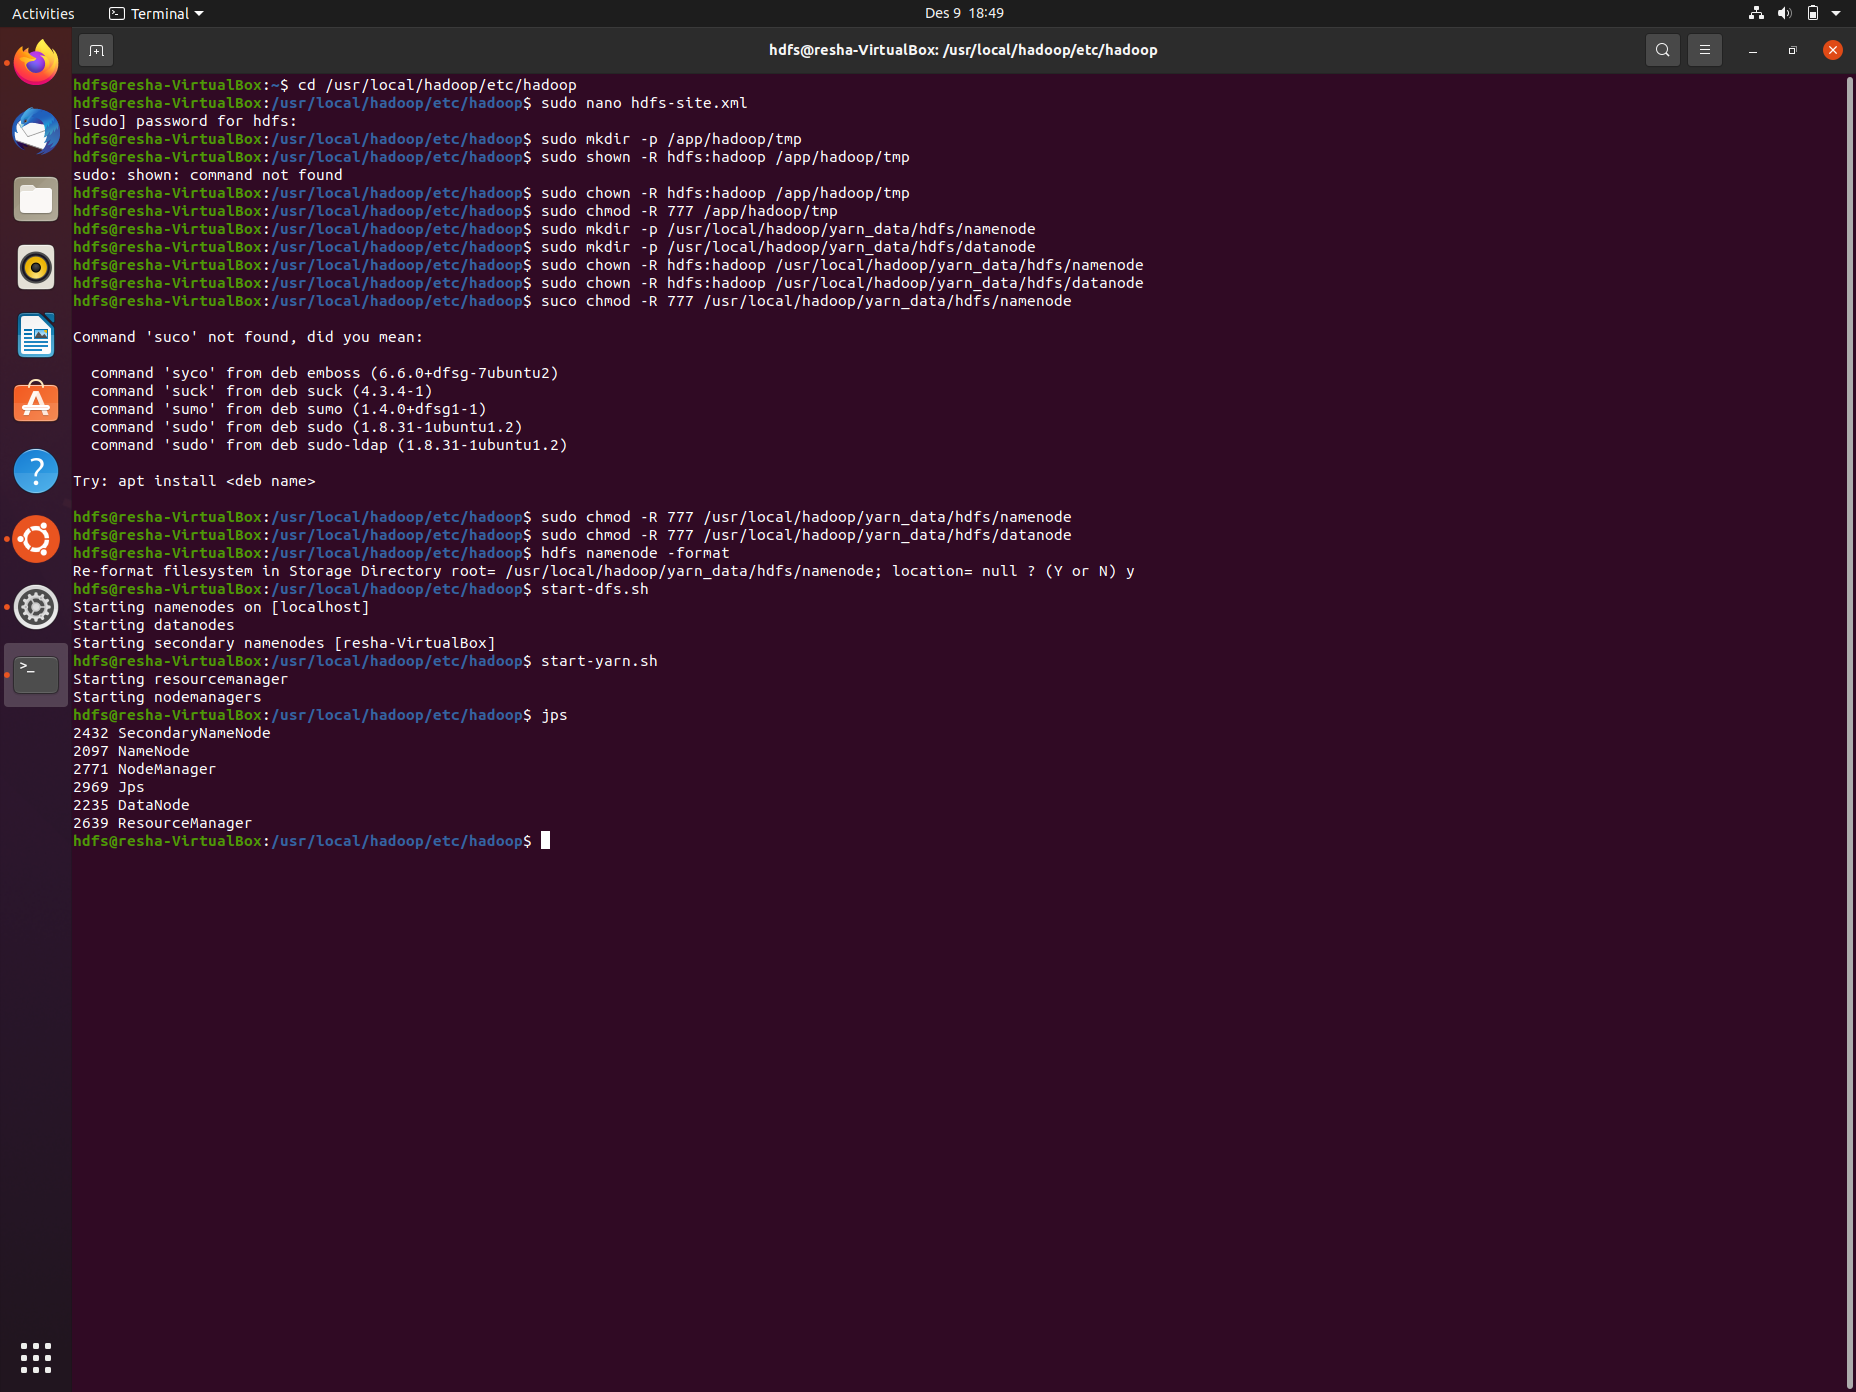
\includegraphics[width=.9\textwidth]{ReshaRussita/jpshadoopservice-resha}
\caption{cek services hadoop dengan jps}
\label{gam:perkuliahan-22-09}
\end{figure}

\begin{figure}[!ht]
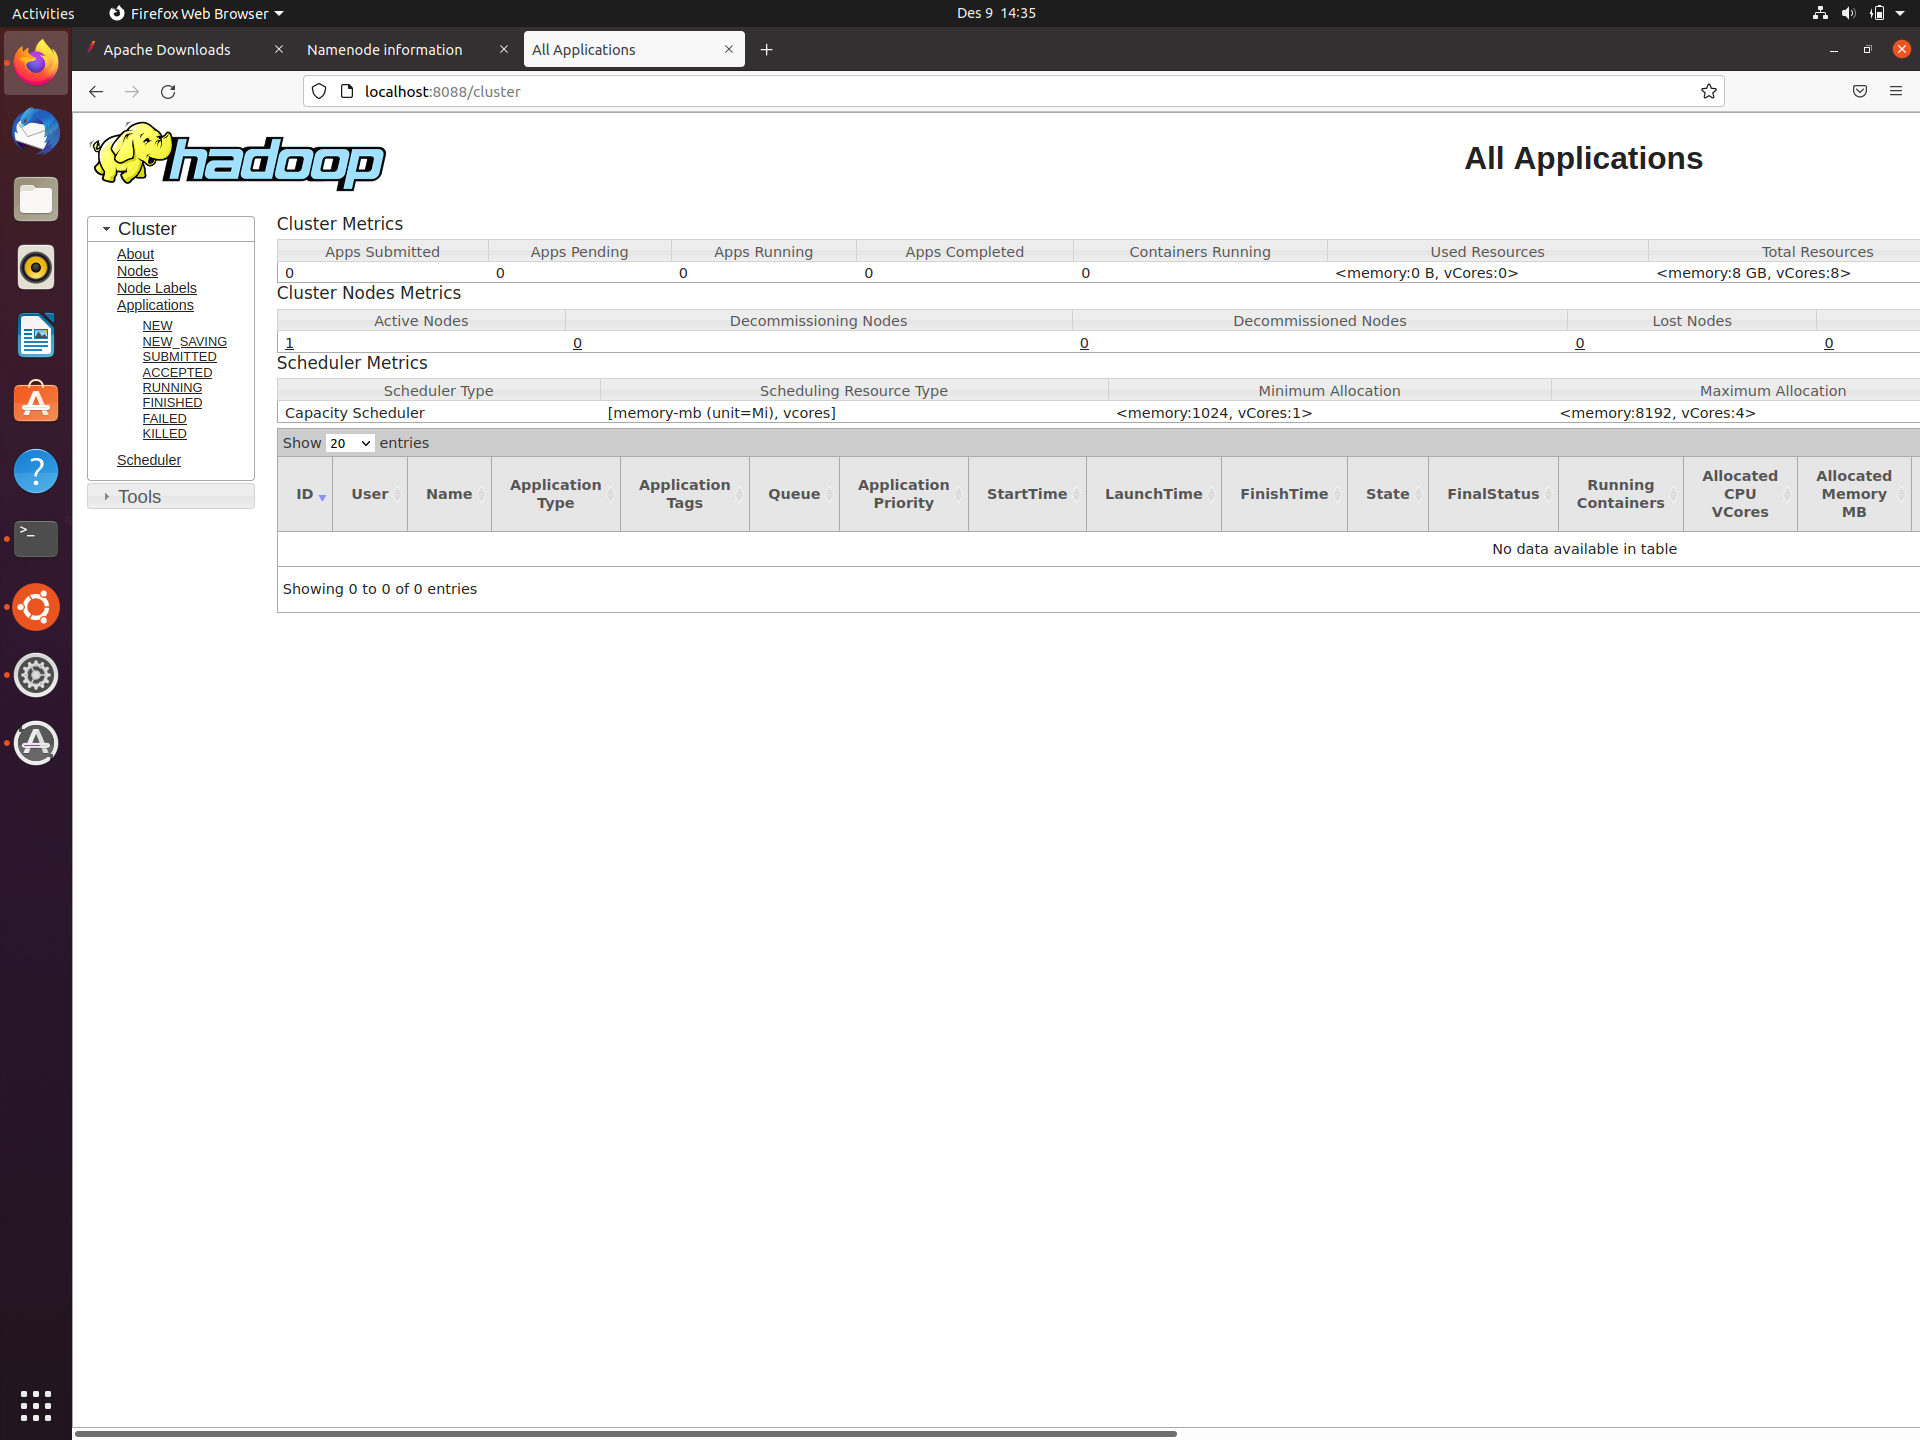
\includegraphics[width=.9\textwidth]{ReshaRussita/localhost8088-resha}
\caption{local host 8088 akses}
\label{gam:perkuliahan-22-09}
\end{figure}

\begin{figure}[!ht]
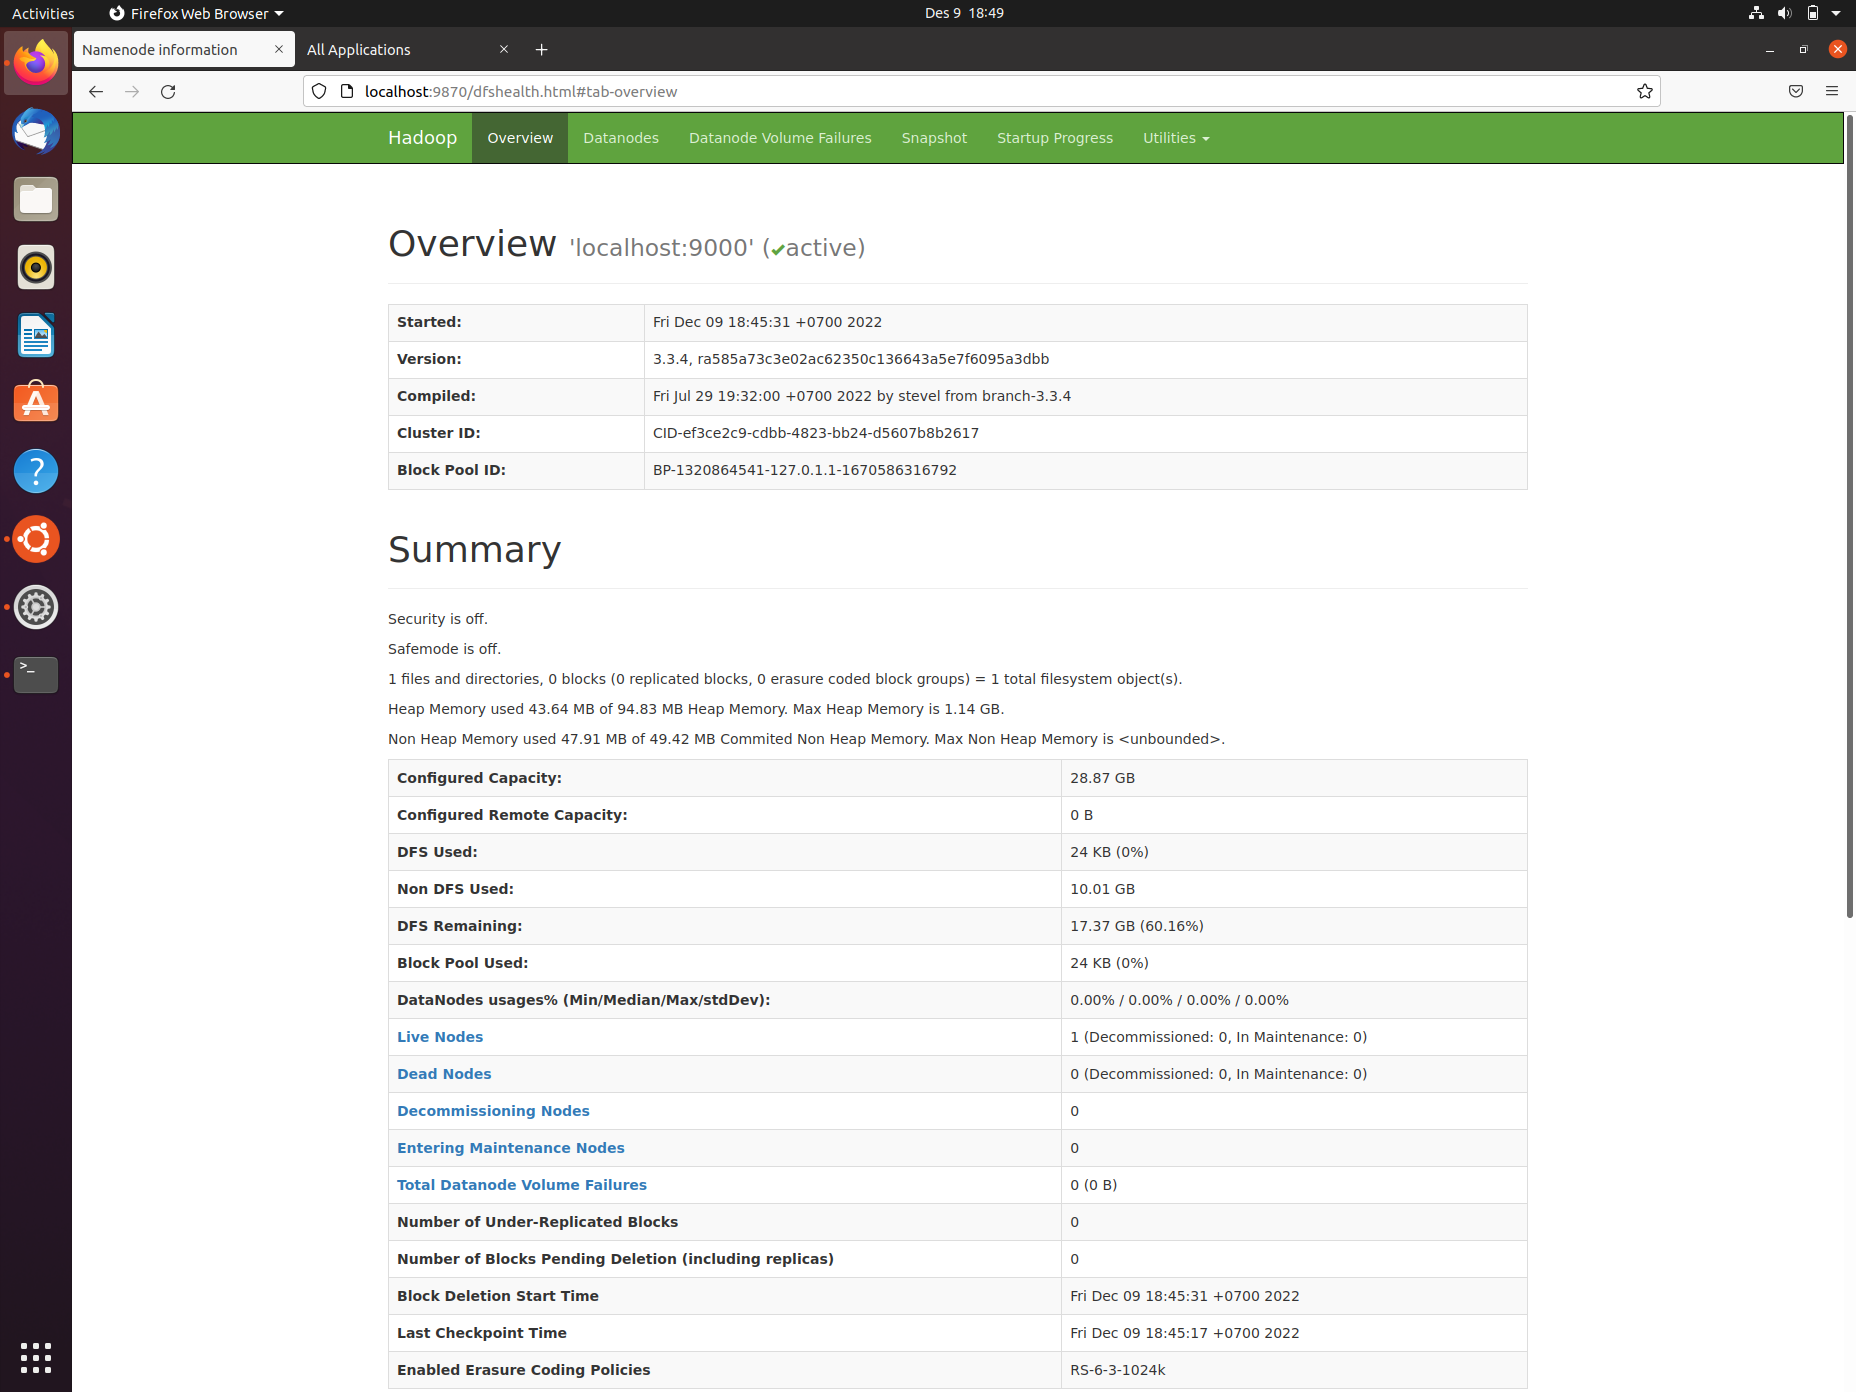
\includegraphics[width=.8\textwidth]{ReshaRussita/localhost9870-resha}
\caption{local host 9870 akses}
\label{gam:perkuliahan-22-09}
\end{figure}

\newpage
\item Kesimpulan
\newline Pada Instalasi Apache Hadoop membutuhkan ruang yang cukup besar untuk mengekstrak file Apache Hadoop. Penginstalaan Apache Hadoop harus dilakukan sesuai step, begitu juga pada saat konfigurasi. Konfigurasi ini bertujuan untuk memudahkan user dalam memonitoring ekosistem di dalam Hadoop. Saat mengkonfigurasi terdapat perintah untuk membuat format HDFS yang berfungsi menyimpan suatu data dengan cara membaginya menjadi potong-potongan data yang disebut blok berukuran 64 MB dan kemudian disimpan pada node-node yang tersebar dalam kluster. Node-node yang ada adalah name node dan data node. Sehingga saat mengecek Hadoop service dengan perintah jps, kedua node tersebut harus tersedia sebagai pendukung saat dilakukan akses web browser dengan local host 9870 dan 8088 itu berhasil.
\end{enumerate}


\newday{\textbf{8 Desember 2022} - WordCount bawaan Hadoop}
\begin{enumerate}
\item Kendala dan Solusi
\newline Pada program WordCount bawaan Hadoop, tidak ada kendala yang saya alami.

\begin{figure}[!ht]
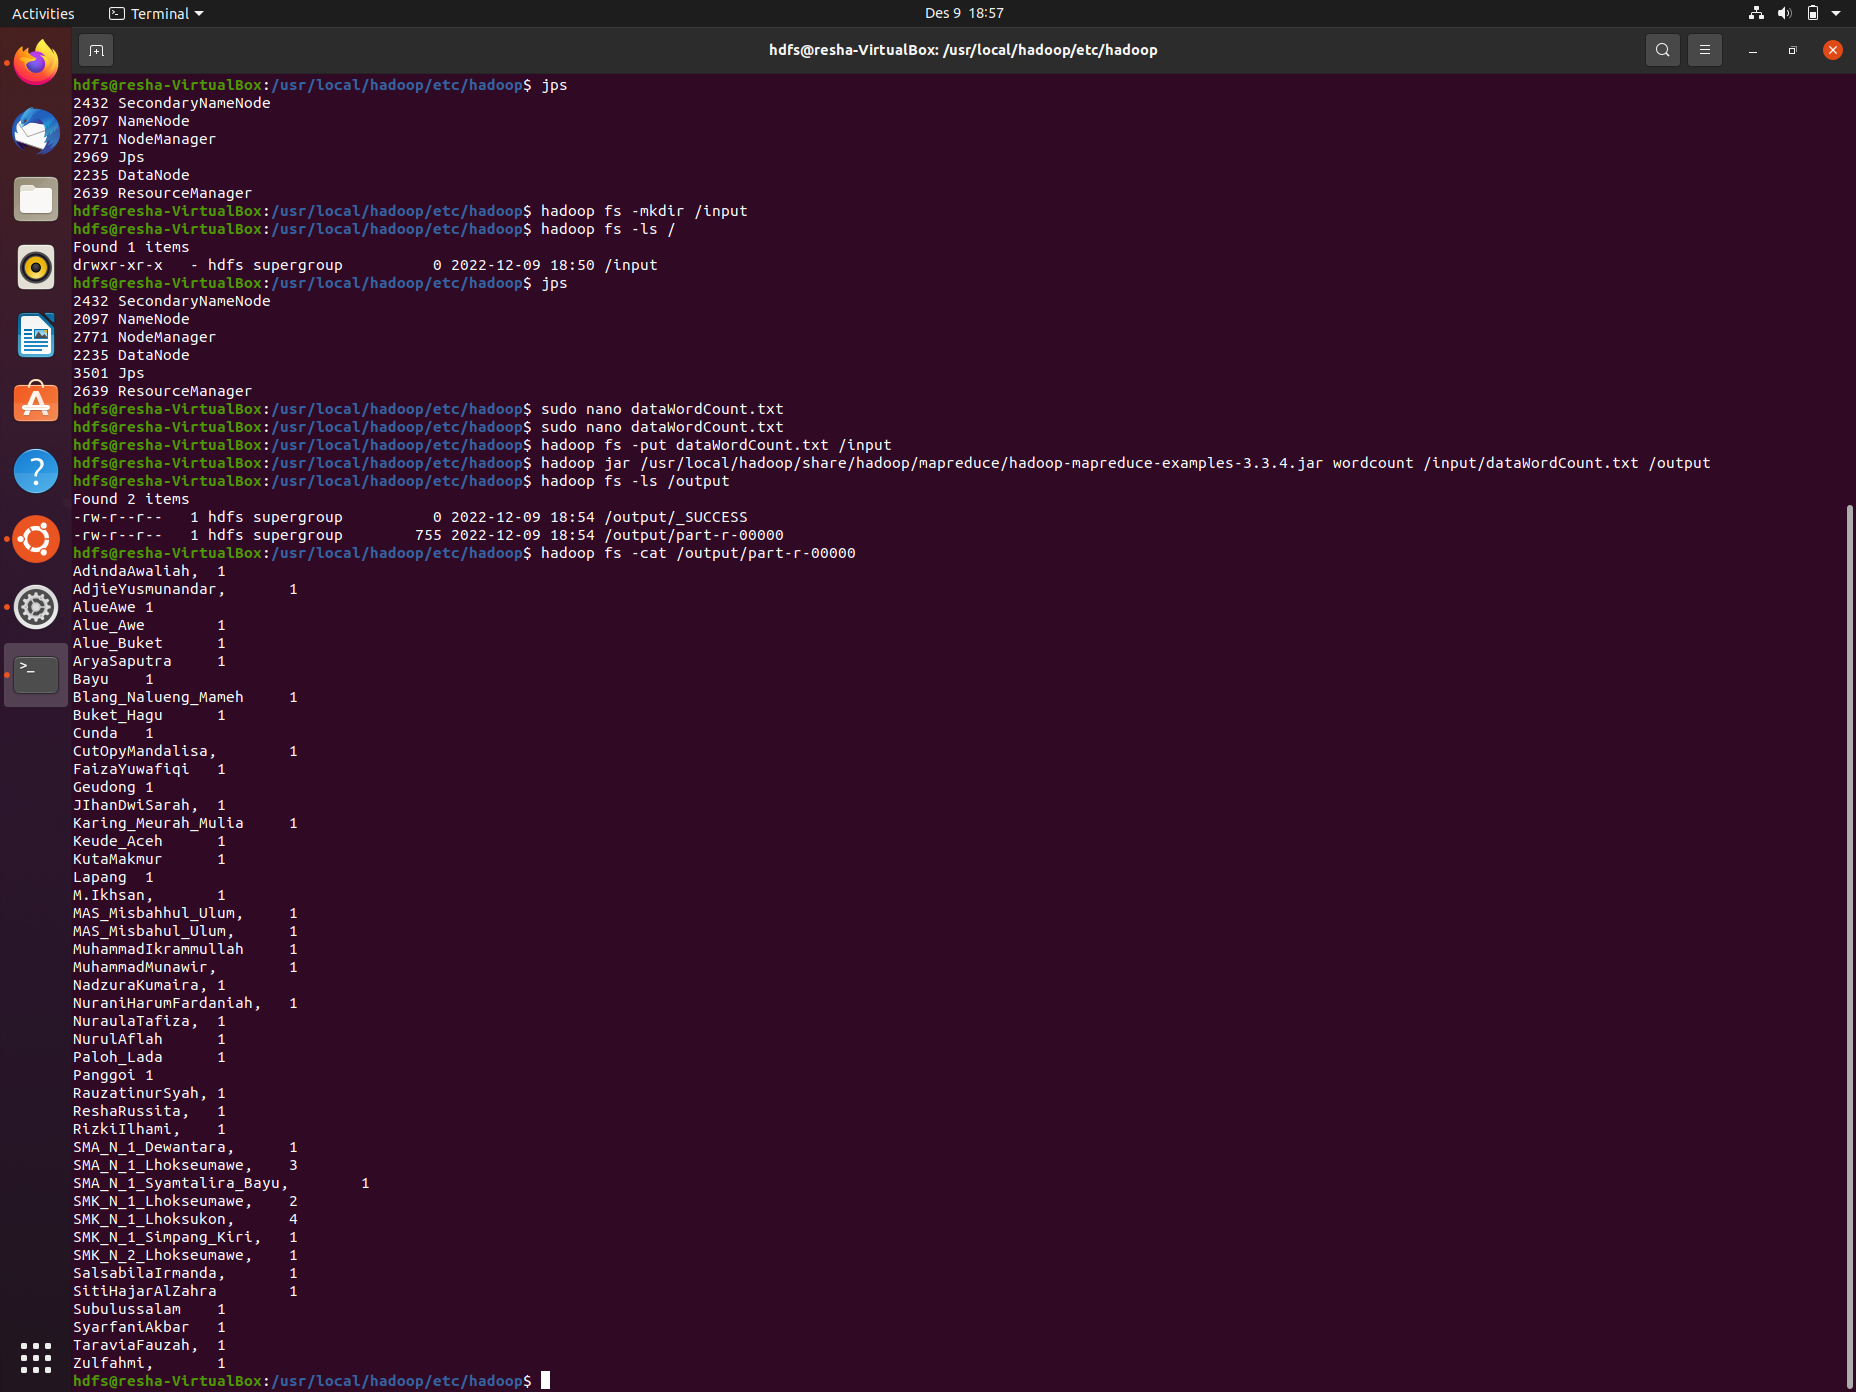
\includegraphics[width=.9\textwidth]{ReshaRussita/langkah6dan7-resha}
\caption{Hasil perhitungan WordCount bawaan Hadoop berdasarkan data output}
\label{gam:perkuliahan-08-12}
\end{figure}

\item Kesimpulan
\newline Pada Hadoop terdapat program untuk menghitung jumlah kata (WordCount) yang ada pada data. Untuk menghitung jumlah kata, saya sebagai praktikan melakukan input data terlebih dahulu, kemudian memprosesnya, sehingga menghasilkan data output. Data output tersebut yang digunakan untuk Hadoop menjalankan programnya yaitu WordCount.
Data yang saya input disini adalah data mahasiswa (nama, asal sekolah, dan alamat). Saat melihat hasil perhitungan pada data output, akan ditampilkan jumlah kata dari tiap-tiap nama, asal sekolah, dan alamat mahasiswa.

\end{enumerate}

\newday{\textbf{9 Desember 2022} - WordCount dengan Java}
\begin{enumerate}
\item Kendala dan Solusi
\newline Pada program WordCount bawaan Java, tidak ada kendala yang saya alami.

\begin{figure}[!ht]
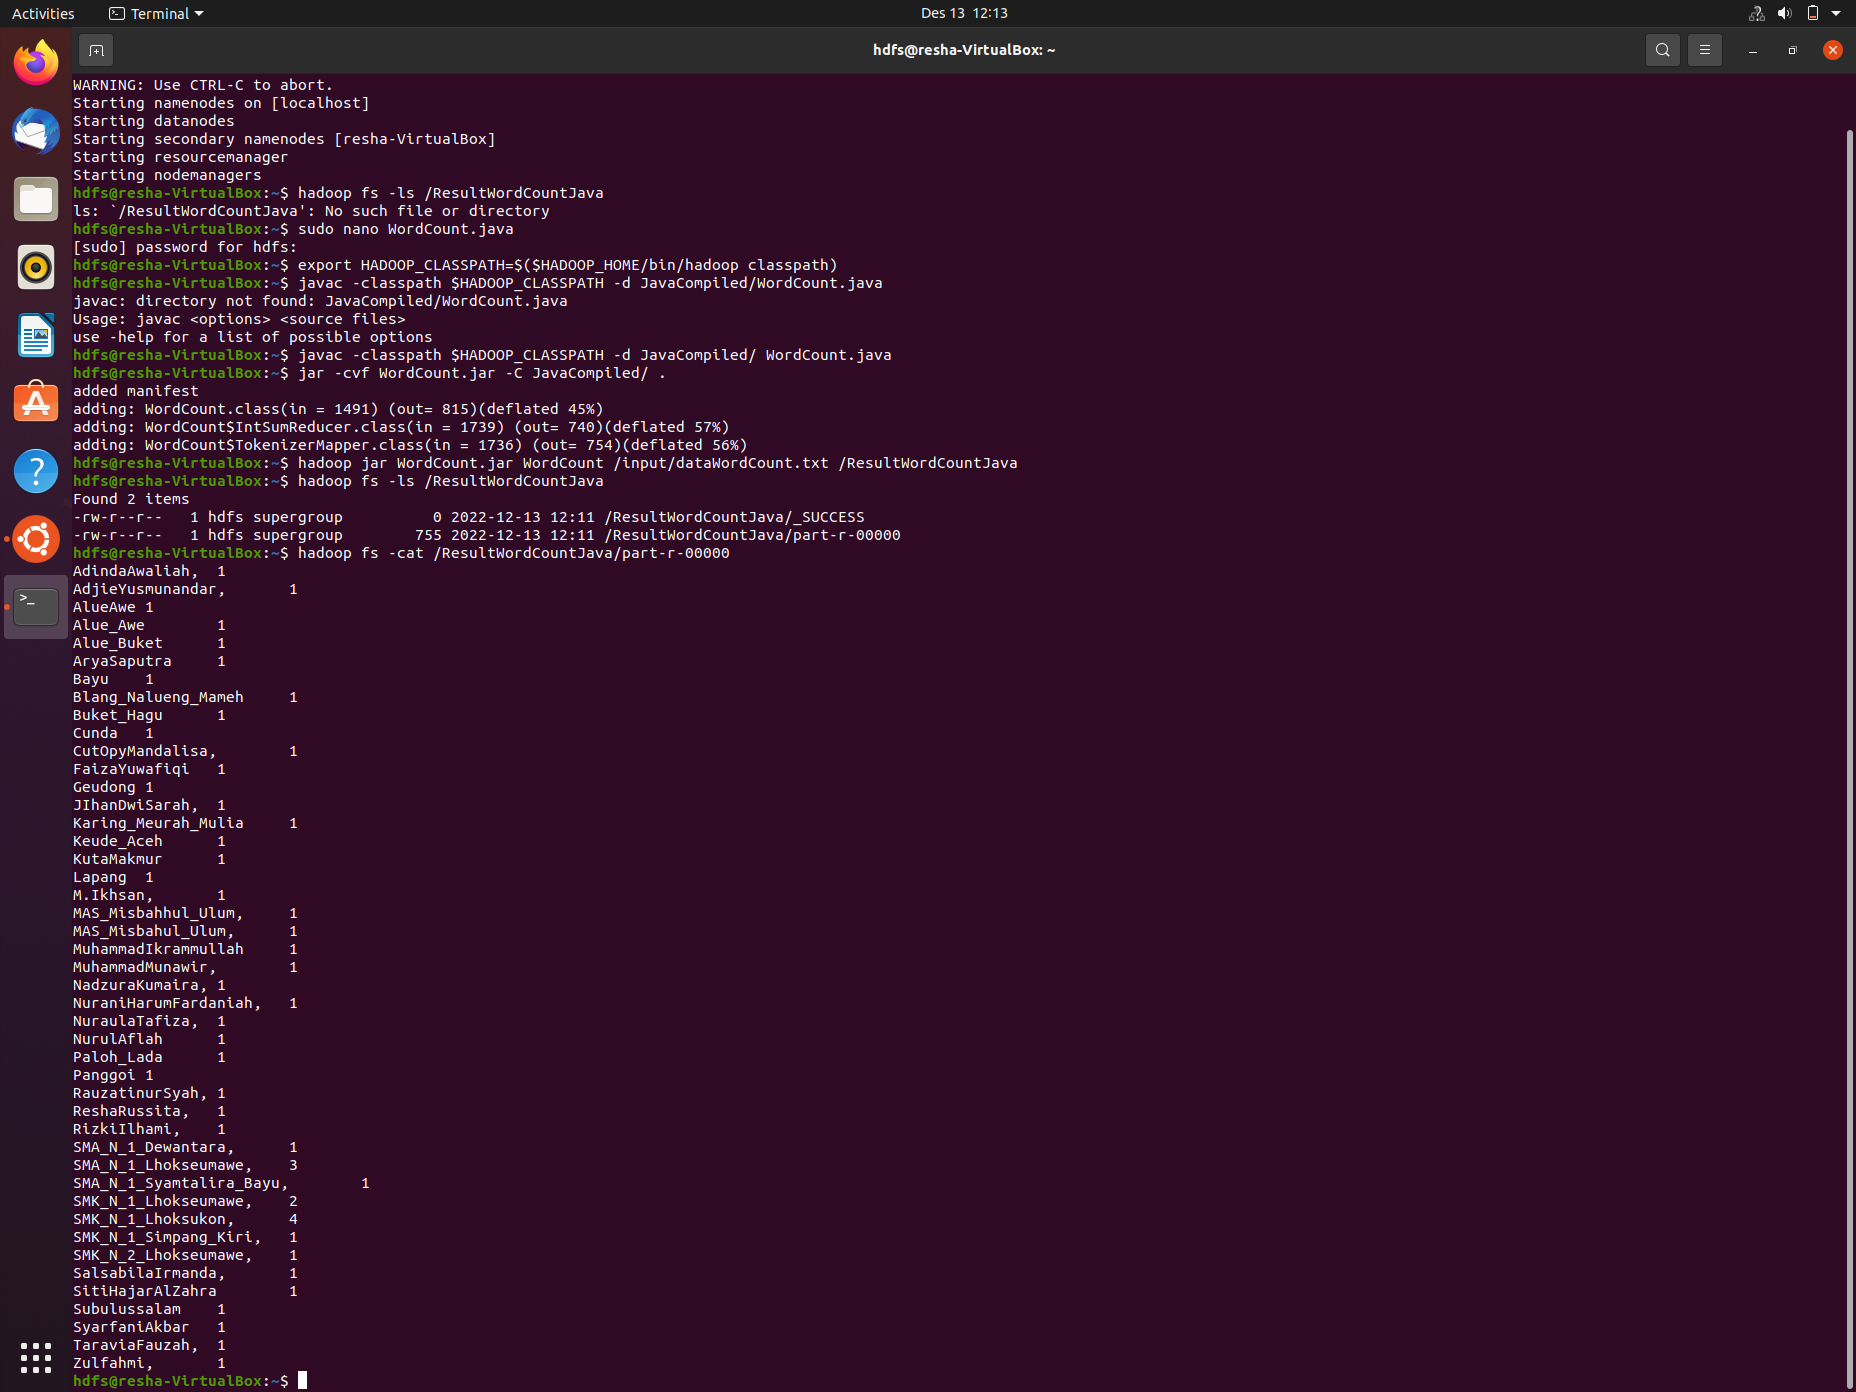
\includegraphics[width=.9\textwidth]{ReshaRussita/langkah9dan10-resha}
\caption{Hasil perhitungan WordCount dengan Java berdasarkan data output}
\label{gam:perkuliahan-08-12}
\end{figure}

\item Kesimpulan
\newline Praktikum ini yaitu menghitung jumlah kata (WordCount) yang ada pada data Java. Proses yang dijalankan mulai dari membuat program dan menyiapkan data untuk WordCount java, kemudian meng-compile program. Program yang dihasilkan sama seperti yang ditampilkan pada WordCount bawaan Hadoop.
\end{enumerate}

\newday{\textbf{15 Desember 2022} - Instalasi Apache PySpark}
\begin{enumerate}
\item Kendala dan Solusi
\newline Pada proses Instalasi Apache PySpark, tidak ada kendala yang saya alami.

\begin{figure}[!ht]
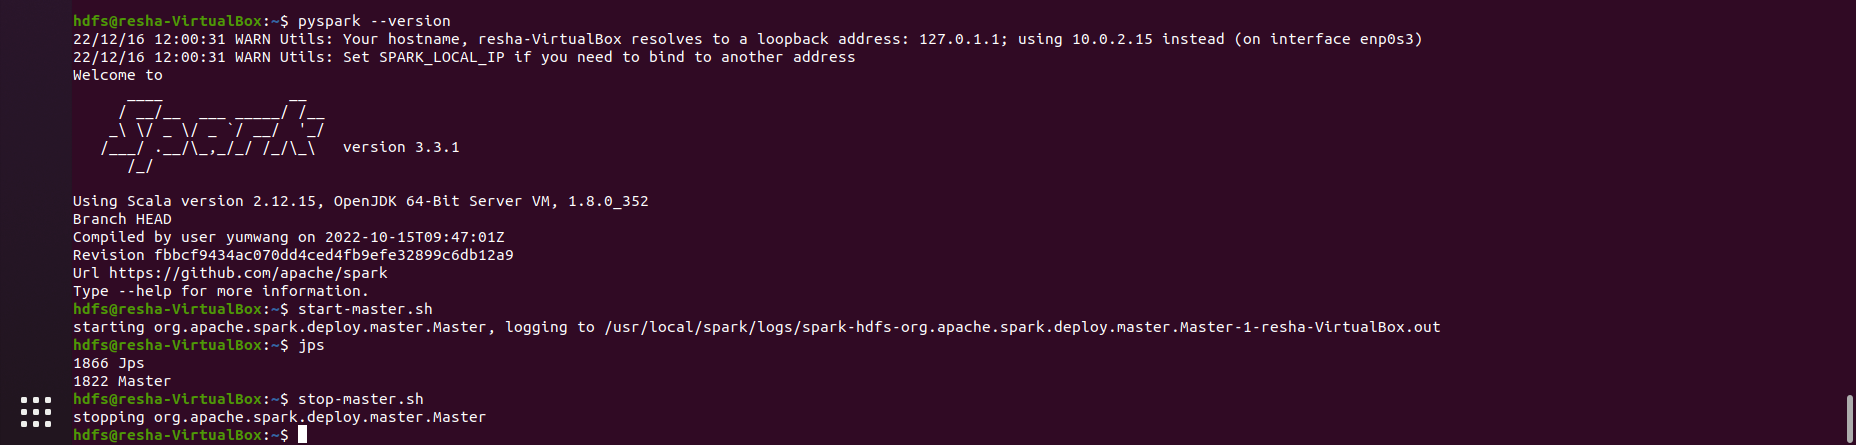
\includegraphics[width=.9\textwidth]{ReshaRussita/langkah5-resha}
\caption{Hasil instalasi Apache PySpark dengan pengecekan versi}
\label{gam:perkuliahan-16-12}
\end{figure}

\item Kesimpulan
\newline Proses instalasi PySpark mirip dengan instalasi hadoop yang dimana perlu menggunakan koneksi yang bukan hotspot atau tethring saat mendownload wget. Untuk memverifikasi hasil instalasi menggunakan perintah pyspark --version. Sama hal-nya saat menjalankan hdfs, untuk menjalankan pyspark juga menggunakan perintah start dan stop. Jika pada hdfs menggunakan perintah start-all.sh, maka pada pyspark menggunakan perintah start-master.sh. Apache Spark adalah sebuah framework komputasi yang dapat digunakan untuk mengakses data, memproses data, menanyakan data serta menganalisis big data. 

\end{enumerate}

\newday{\textbf{16 Desember 2022} - WordCount Hadoop dengan Python}
\begin{enumerate}
\item Kendala dan Solusi
\newline Pada program WordCount Hadoop dengan Python terdapat kendala yang saya alami. Hal ini terjadi karena kekeliruan pada modul. Solusi yang saya lakukan adalah mengupdate ulang modul yang diberikan.

\begin{figure}[!ht]
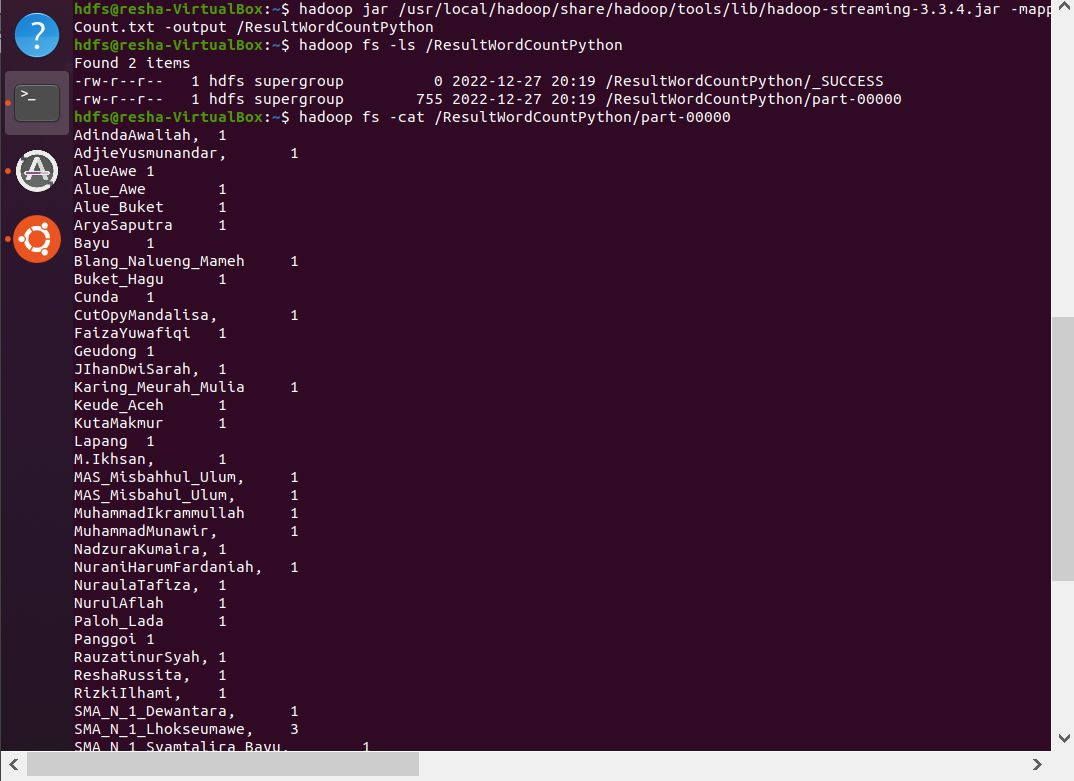
\includegraphics[width=.9\textwidth]{ReshaRussita/langkah8dan9python}
\caption{Hasil perhitungan WordCount Hadoop dengan Python}
\label{gam:perkuliahan-22-12}
\end{figure}

\item Kesimpulan
\newline Pada Hadoop terdapat program untuk menghitung jumlah kata (WordCount) yang ada pada data. Untuk menghitung jumlah kata, saya sebagai praktikan melakukan input data terlebih dahulu, kemudian memprosesnya, sehingga menghasilkan data output. Input data atau kalimat disesuaikan dengan modul dengan bantuan perintah echo. Sehingga output merupakan perhitungan kata dari tiap kata pada kalimat yang ada pada echo. 
Namun disini saya sebagai praktikan menghitung jumlah kata pada dataWordCount.txt dengan python yang berisi jumlah kata nama mahasiswa, asal sekolah, dan alamat.

\end{enumerate}

\newday{\textbf{22 Desember 2022} - WordCount Hadoop dengan PySpark}
\begin{enumerate}
\item Kendala dan Solusi
\newline Pada program WordCount Hadoop dengan PySpark tidak ada kendala yang saya alami.

\begin{figure}[!ht]
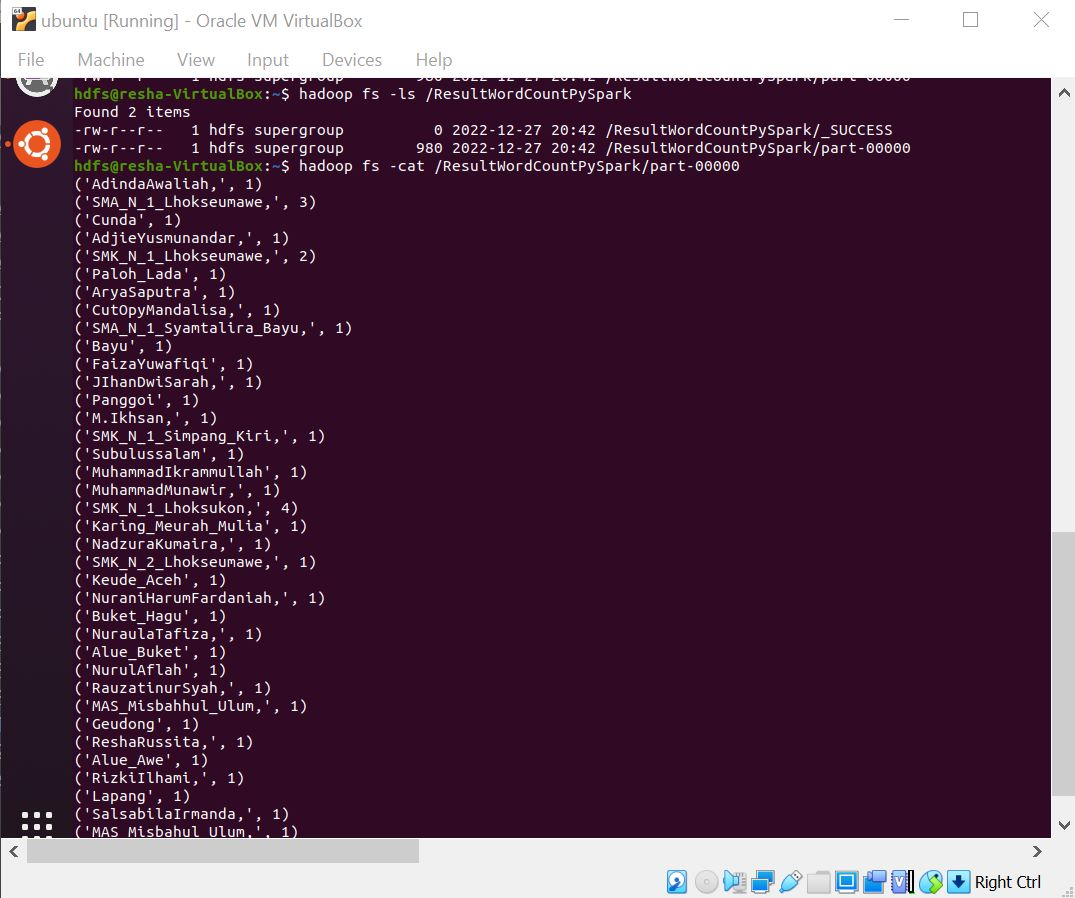
\includegraphics[width=.9\textwidth]{ReshaRussita/langkah6dan7pyspark}
\caption{Hasil perhitungan WordCount Hadoop dengan PySpark}
\label{gam:perkuliahan-22-12}
\end{figure}

\item Kesimpulan
\newline Pada Hadoop terdapat program untuk menghitung jumlah kata (WordCount) yang ada pada data. 
Namun disini saya sebagai praktikan menghitung jumlah kata pada WordCount.py dengan pyspark yang berisi jumlah kata nama mahasiswa, asal sekolah, dan alamat. Sama seperti sebelumnya, namun dilengkapi dengan tanda (' ')

\end{enumerate}

\newday{\textbf{23 Desember 2022} - Tugas Individu}
\begin{enumerate}
\item Kendala dan Solusi
\newline Pada tugas individu, tidak banya kendala yang saya alami. Kendala yang terjadi adalah hanya kekeliruan pada perintah saja. Solusi yang saya lakukan adalah melakukan teliti kembali pada perintah yang saya buat sebelumnya.

\begin{figure}[!ht]
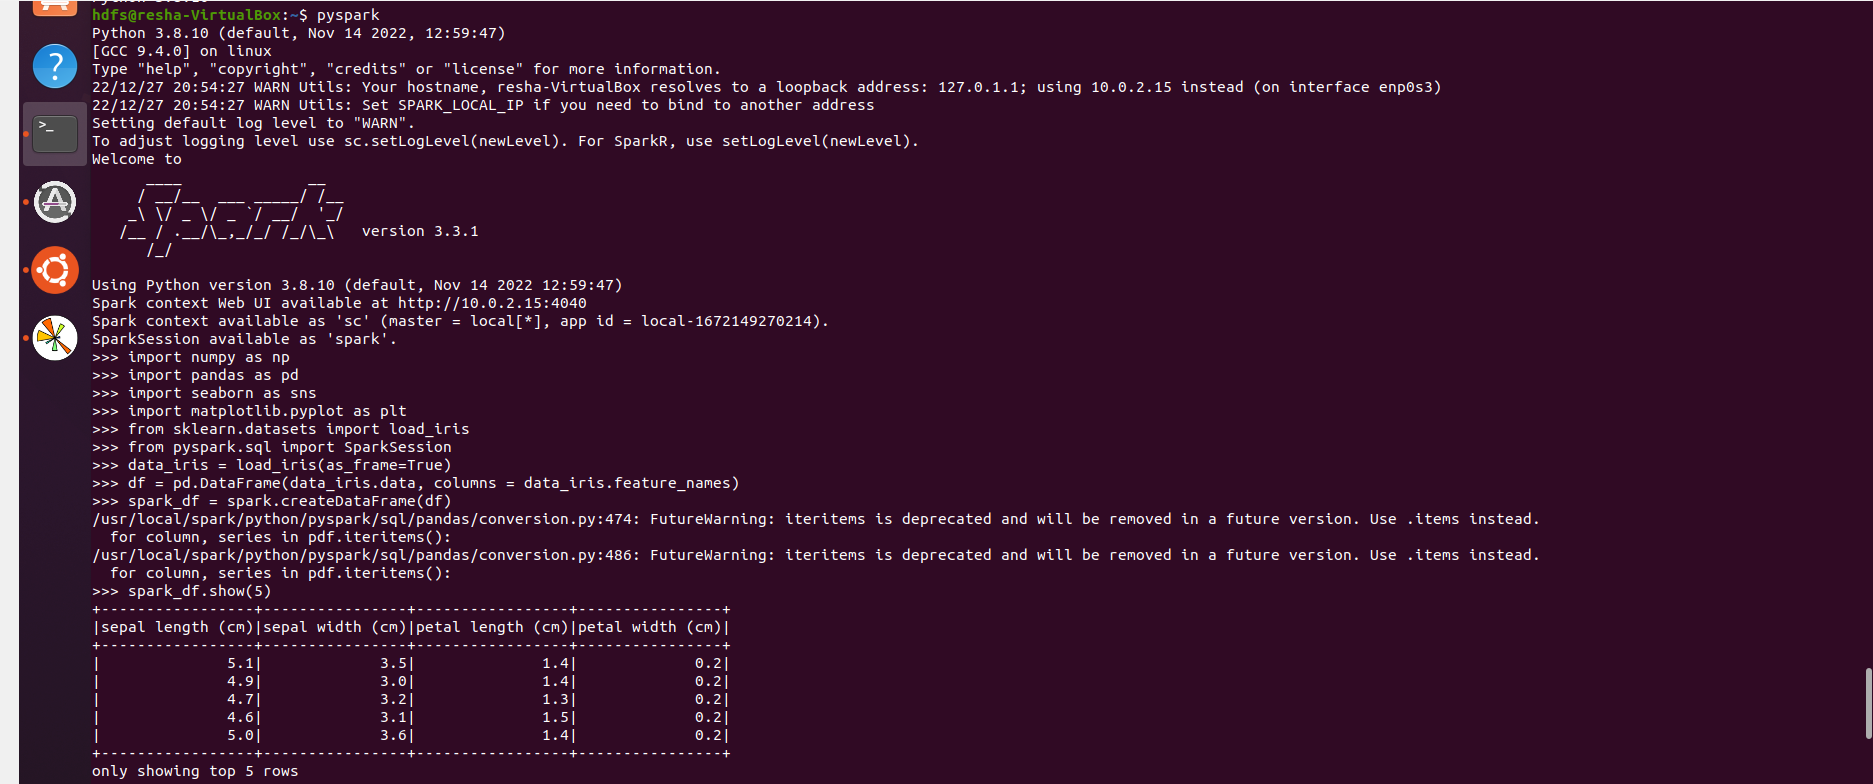
\includegraphics[width=.9\textwidth]{ReshaRussita/tabelciri}
\caption{ciri-ciri dari bunga iris berdasarkan sepal dan petal}
\label{gam:perkuliahan-23-09}
\end{figure}

\begin{figure}[!ht]
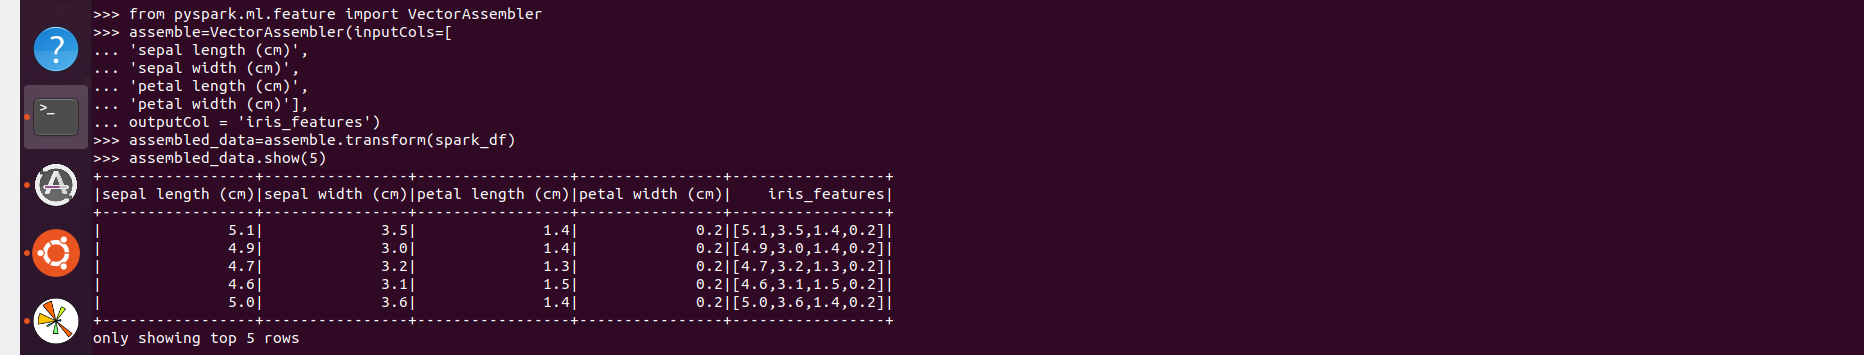
\includegraphics[width=.9\textwidth]{ReshaRussita/tabelvektor}
\caption{vektor bunga iris yang dihasilkan dari ciri-ciri yang telah diinput}
\label{gam:perkuliahan-23-09}
\end{figure}

\begin{figure}[!ht]
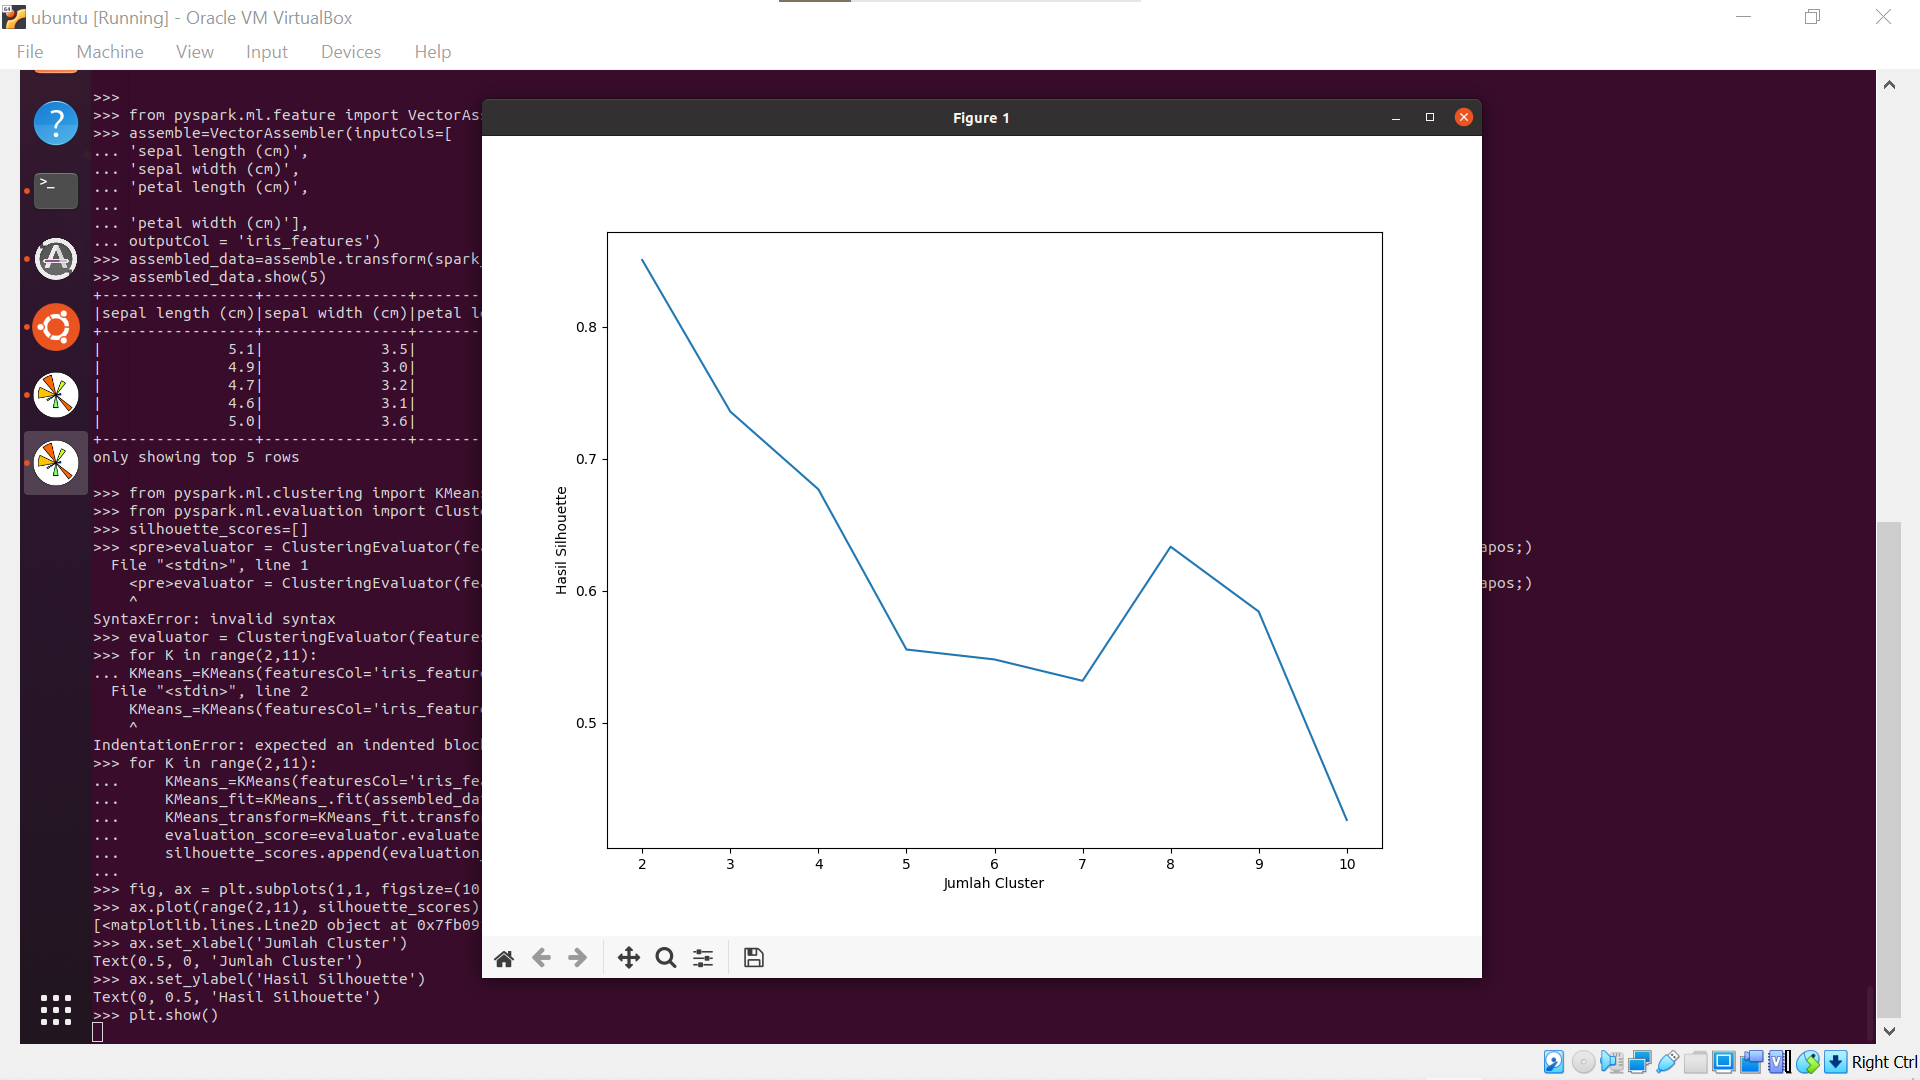
\includegraphics[width=.8\textwidth]{ReshaRussita/grafikjumlahclusterdanhasilsilhouette}
\caption{grafik jumlah cluster dan hasil silhouette dari software metaploit}
\label{gam:perkuliahan-23-09}
\end{figure}

\begin{figure}[!ht]
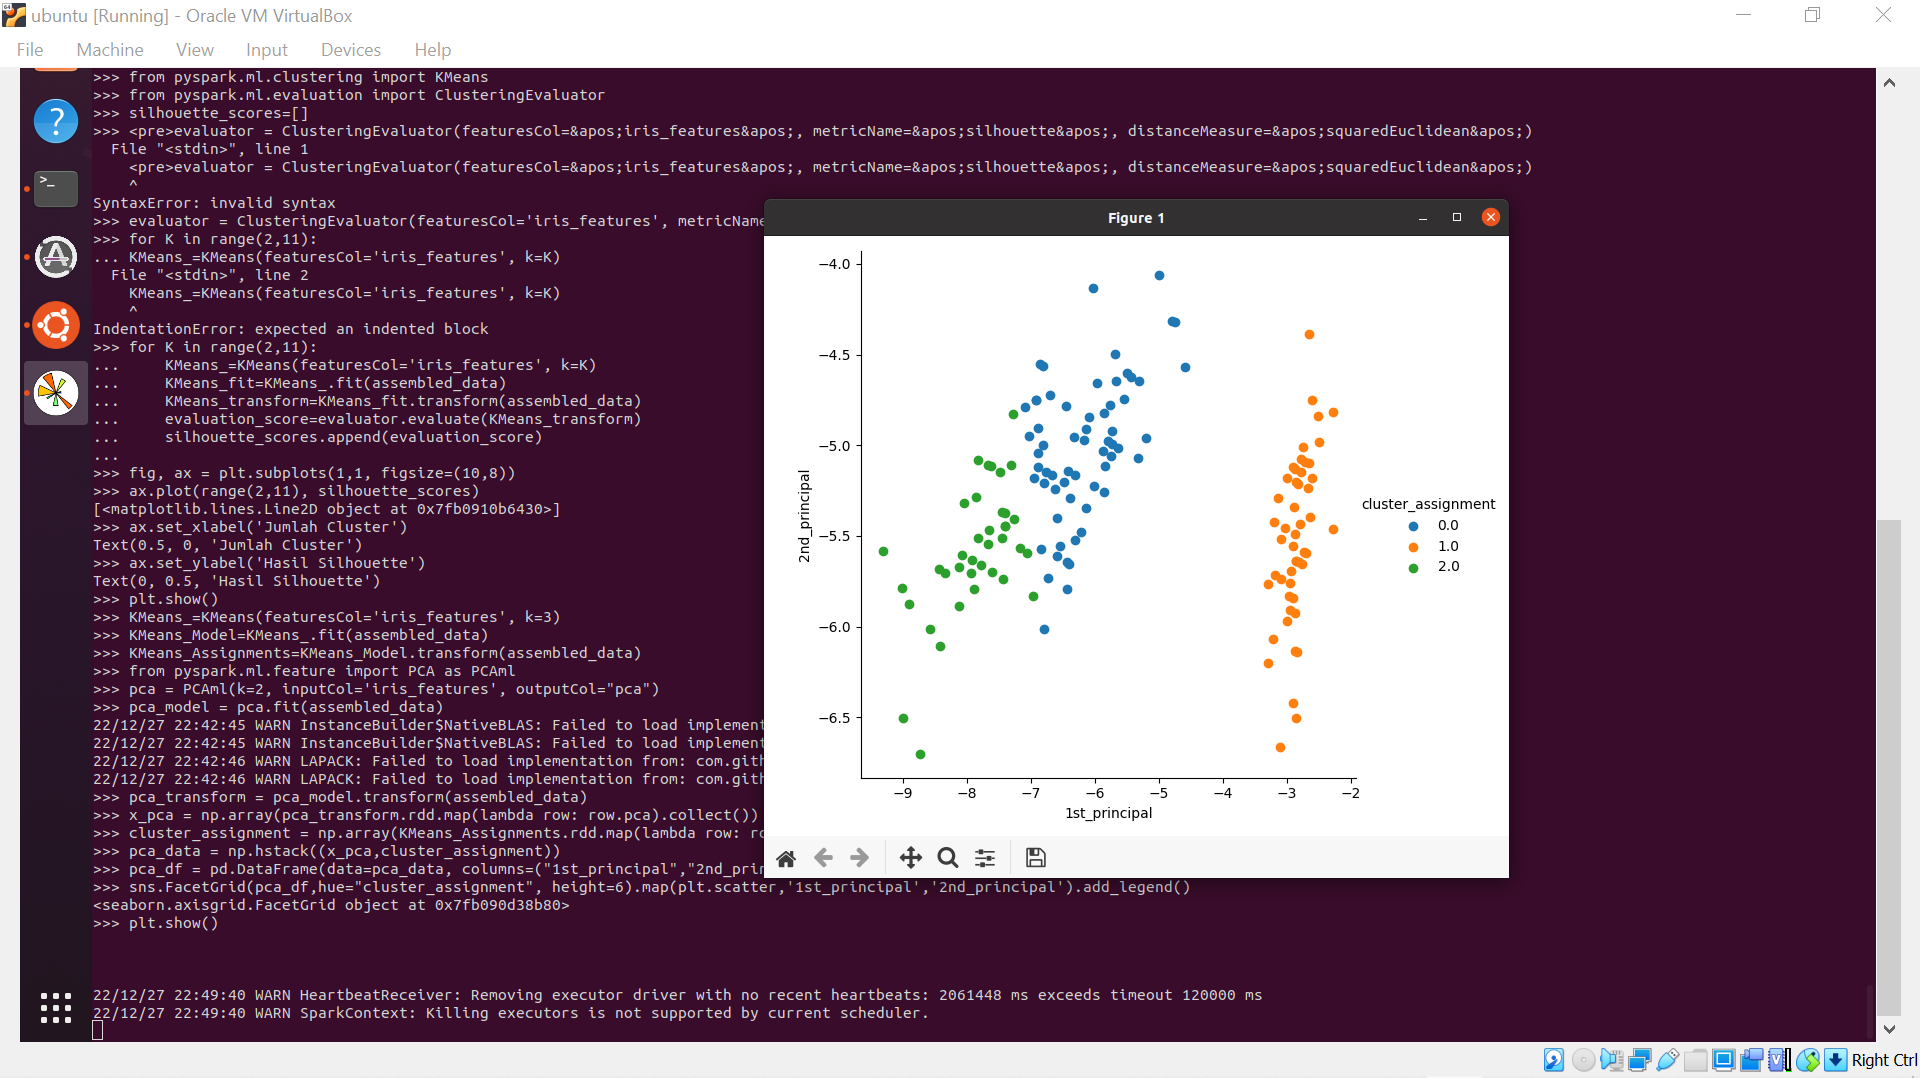
\includegraphics[width=.8\textwidth]{ReshaRussita/grafikclusterassignment}
\caption{grafik cluster assignment dari software metaploit}
\label{gam:perkuliahan-23-09}
\end{figure}

\item Kesimpulan
\newline Pada tugas individu yaitu menampilkan grafik mengenai bunga iris berdasarkan ciri-ciri yang telah diinput yaitu lebar sepal, tinggi sepal, lebar petal, dan tinggi petal. Hasil dari ciri-ciri tersebut menghasilkan vektor yang berbeda-beda mengenai bunga iris. Terdapat 5 vektor di dalamnya berdasarkan baris ciri-ciri yang berbeda-beda. 
\newline Grafik pertama yang dihasilkan adalah grafik mengenai jumlah cluster dan hasil silhouette yaitu metode yang digunakan untuk menempatkan suatu objek pada cluster. 
\newline Grafik kedua yang dihasilkan yaitu perhitungan jumlah titik pada cluster 0, cluster 1, dan cluster 2. 

\end{enumerate}

\newday{\textbf{23 Desember 2022} - Tugas Kelompok 4}
\begin{enumerate}
\item Kendala dan Solusi
\newline Pada tugas kelompok membuat file python yang dapat dijalankan dengan spark-submit, tidak ada kendala yang terlalu berat di dalamnya. Hanya saja terdapat error pada proses pemunculan grafik terakhir mengenai cluster assignment. 
\newline solusi yang kami lakukan adalah melakukan pengecekkan ulang pada program yang ada pada file python

\item Kesimpulan
\newline Pada tugas kelompok yaitu membuat file python yang dapat dijalankan dengan spark-submit, kami dari kelompok 4 berhasil menyelesaikan tugas ini.
\newline Berikut alur atau langkah-langkah praktikum tugas kelompok ini:
1) Membuat direktori baru di dalam hdfs. Direktori ini kami beri nama FolderPyspark. Kemudian masuk ke direktori tersebut, dan membuat file python untuk mengisi program. File python ini kami beri nama pysparkbigdata.py 

\begin{figure}[!ht]
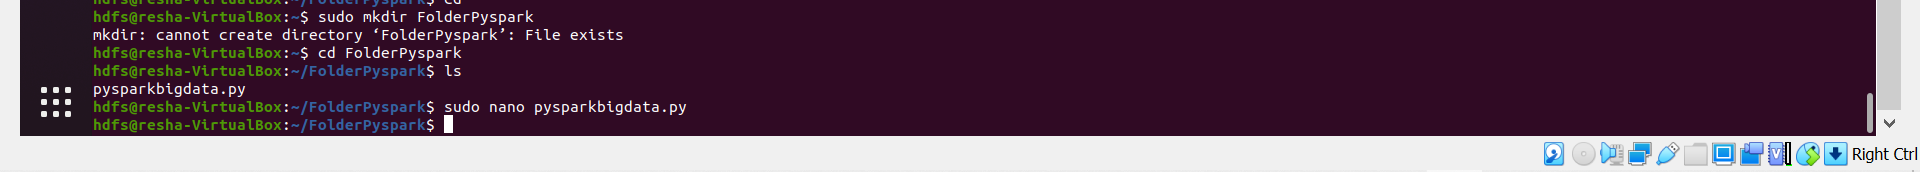
\includegraphics[width=.9\textwidth]{TugasKelompok/Kelompok4/direktoribarudanfilepython}
\caption{Direktori baru dan file python}
\label{gam:perkuliahan-23-09}
\end{figure}

2) Mengisi program seperti yang ada pada tugas individu ke dalam file python yang telah dibuat sebelumnya yaitu pysparkbigdata.py
\begin{figure}[!ht]
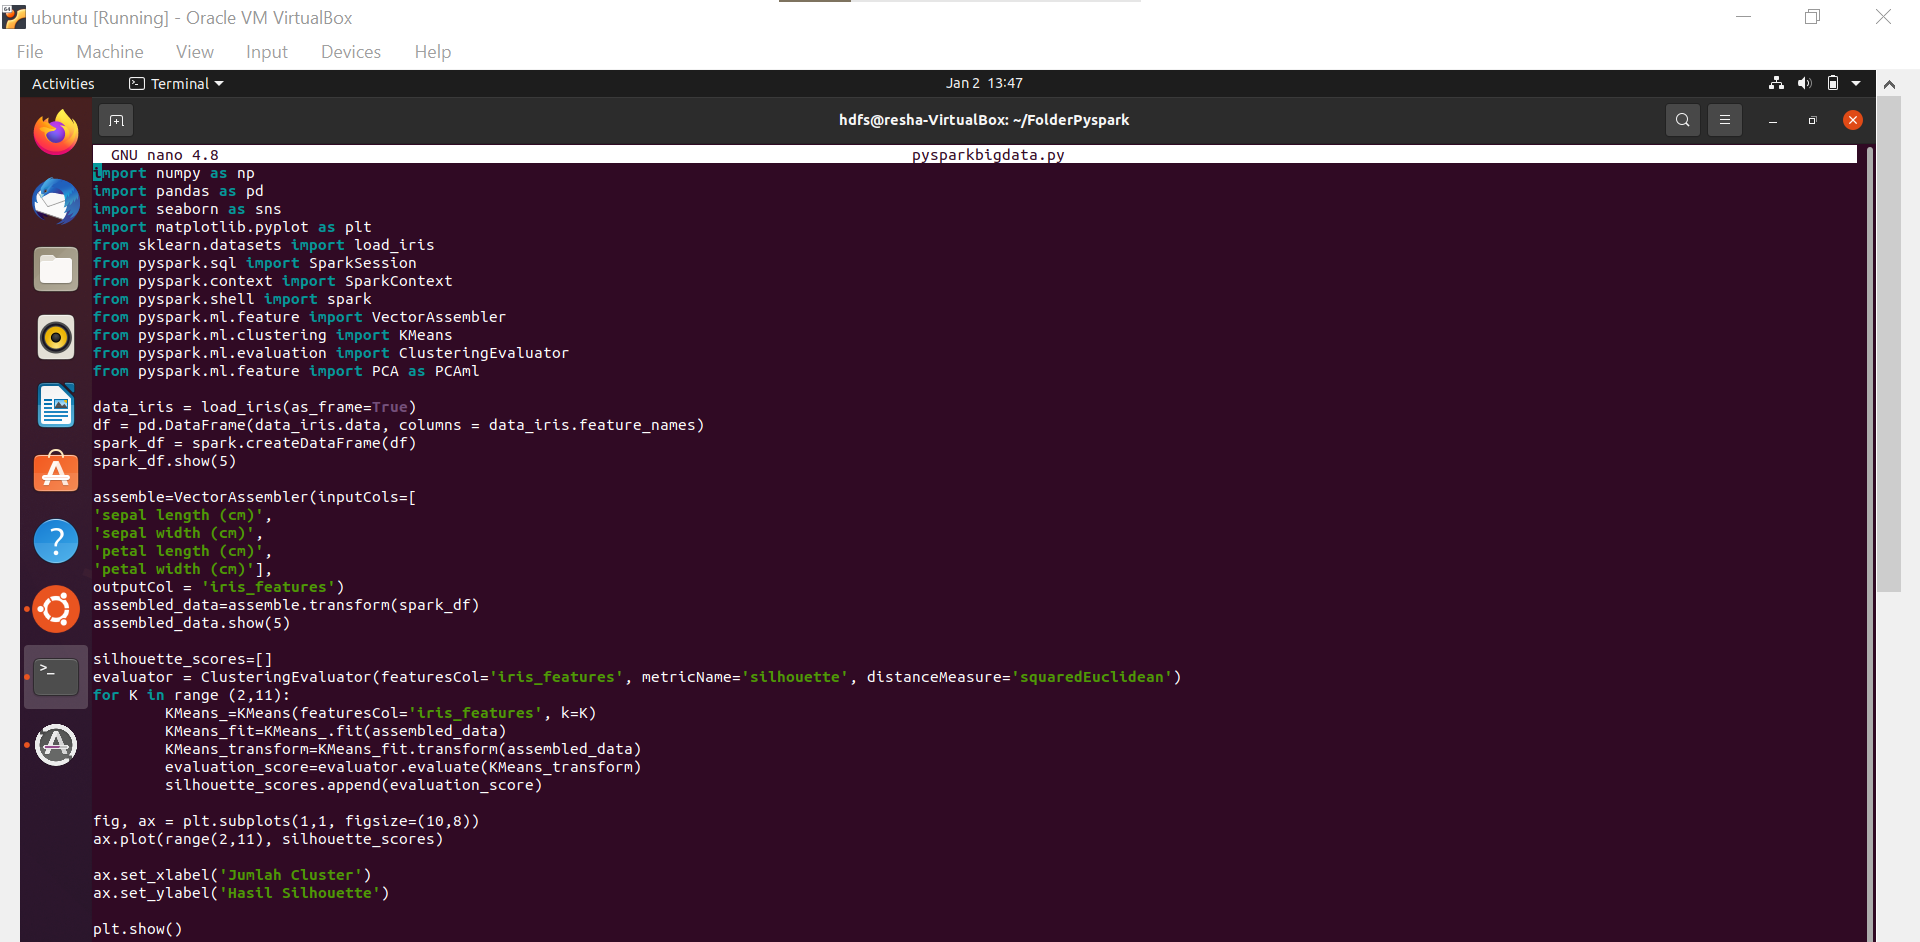
\includegraphics[width=.9\textwidth]{TugasKelompok/Kelompok4/programpython}
\caption{Program file python}
\label{gam:perkuliahan-23-09}
\end{figure}
\begin{figure}[!ht]
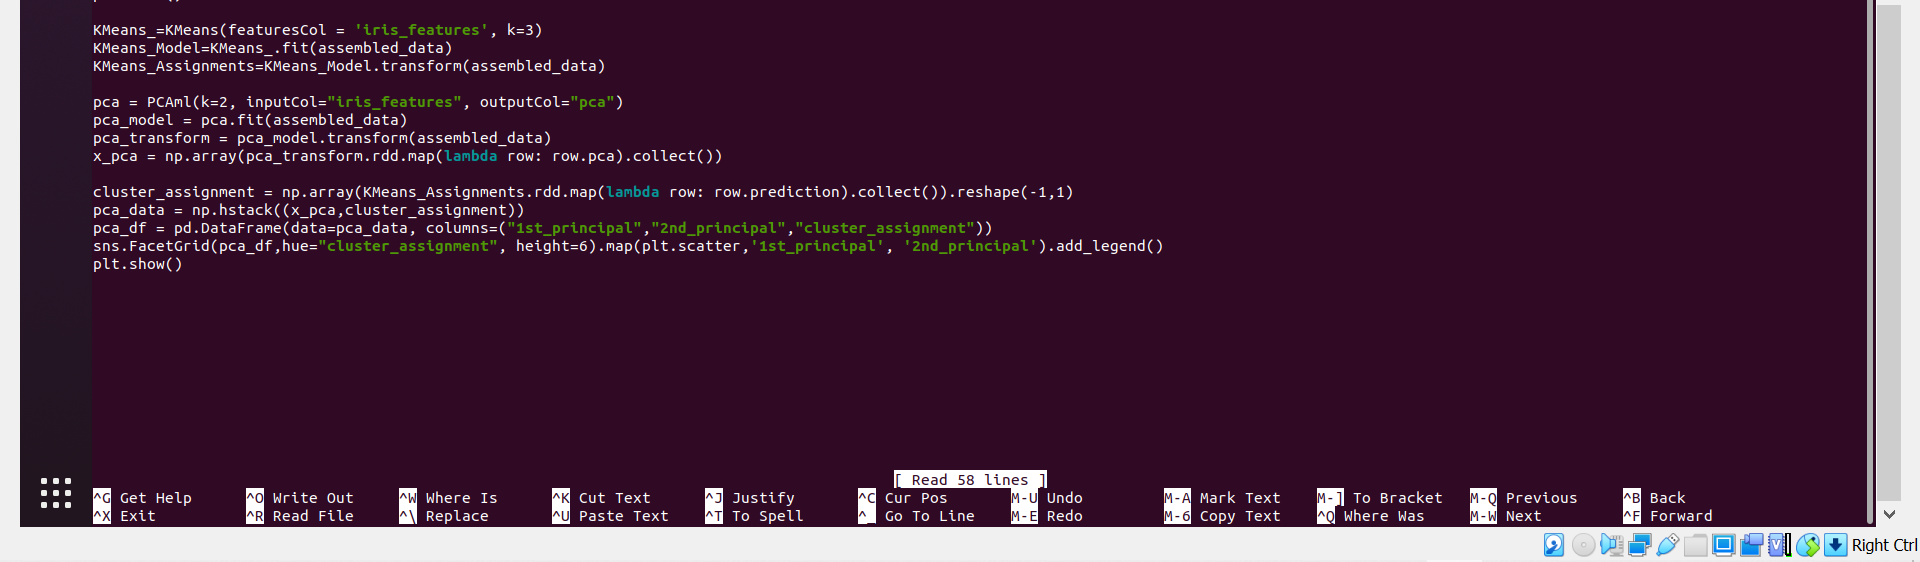
\includegraphics[width=.9\textwidth]{TugasKelompok/Kelompok4/programpython2}
\caption{Program file python}
\label{gam:perkuliahan-23-09}
\end{figure}

3) Menjalankan program tersebut dengan perintah spark-submit pysparkbigdata.py dan tunggu proses selesai. Proses selesai ditandai dengan munculnya 2 tabel mengenal deskripsi bunga iris dan vektor yang dihasilkan dari deskripsi tersebut, juga 2 grafik mengenai jumlah cluster hasil silhouette dan cluster assignment.
\begin{figure}[!ht]
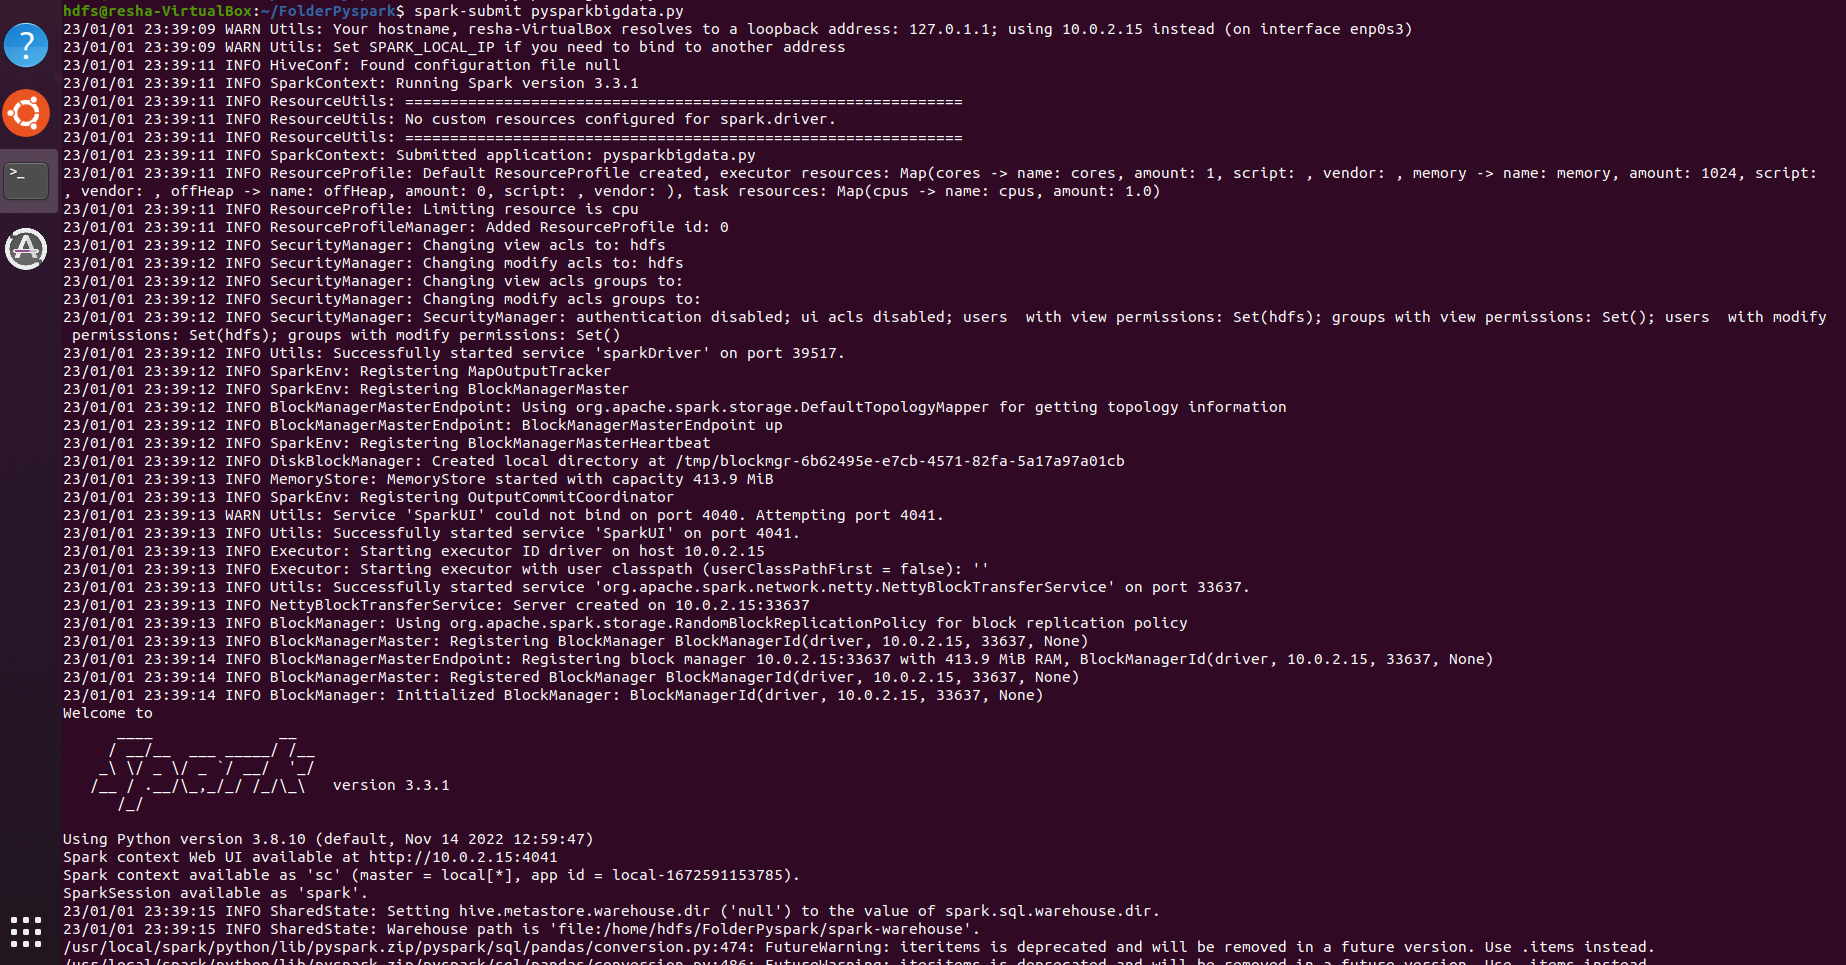
\includegraphics[width=.8\textwidth]{TugasKelompok/Kelompok4/runningdenganpyspark}
\caption{Menjalankan program menggunakan Pyspark}
\label{gam:perkuliahan-23-09}
\end{figure}

4) Melihat hasil yang ditampilkan.
\begin{figure}[!ht]
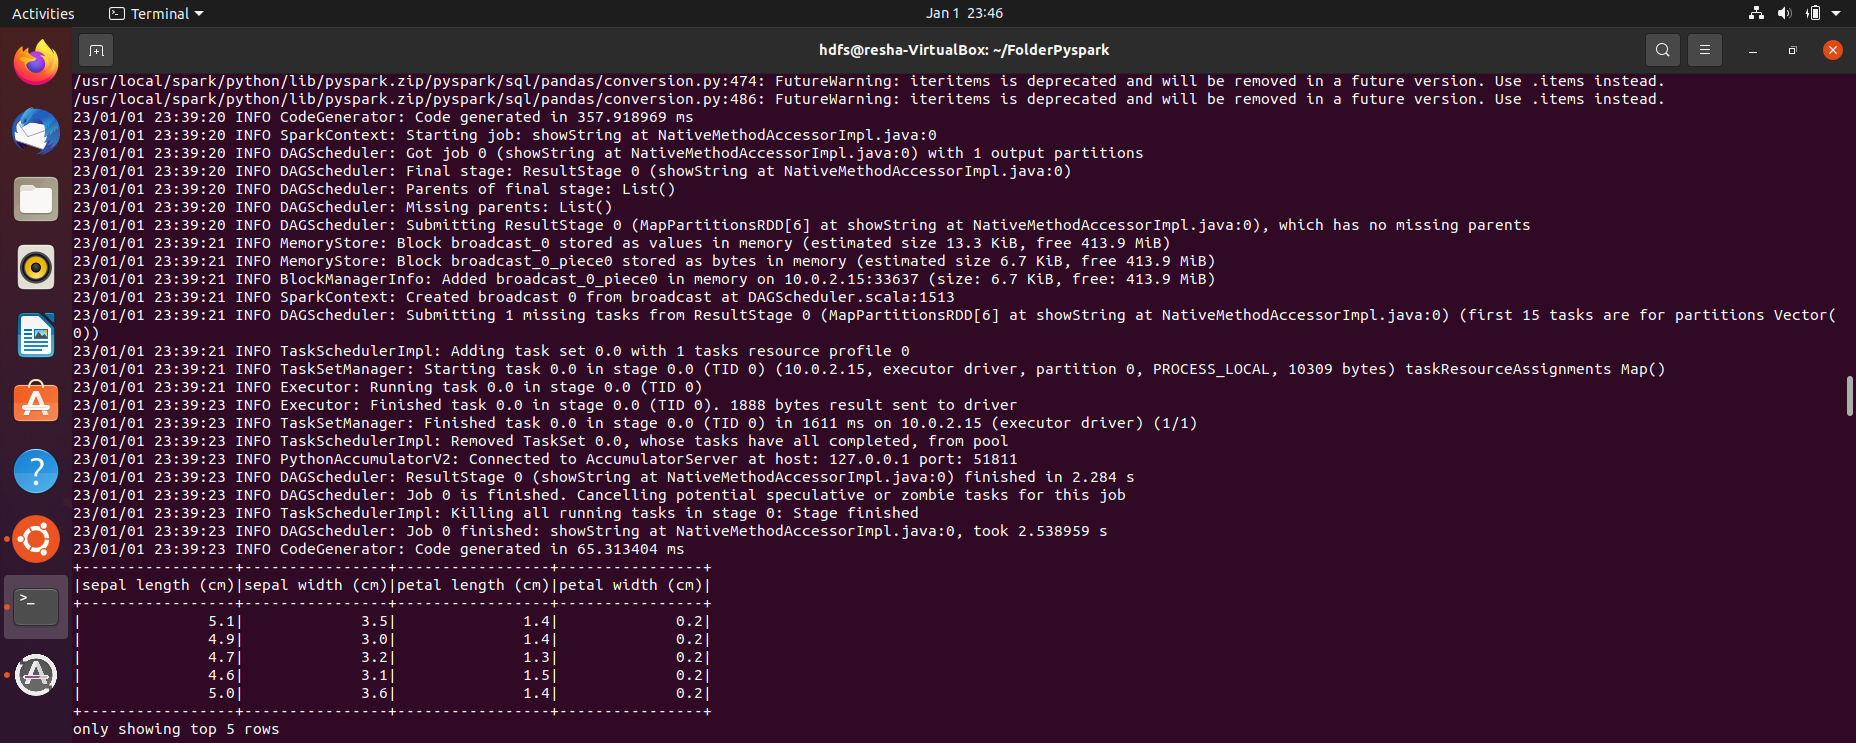
\includegraphics[width=.9\textwidth]{TugasKelompok/Kelompok4/tabelpertama}
\caption{ciri-ciri dari bunga iris berdasarkan sepal dan petal}
\label{gam:perkuliahan-23-09}
\end{figure}
\begin{figure}[!ht]
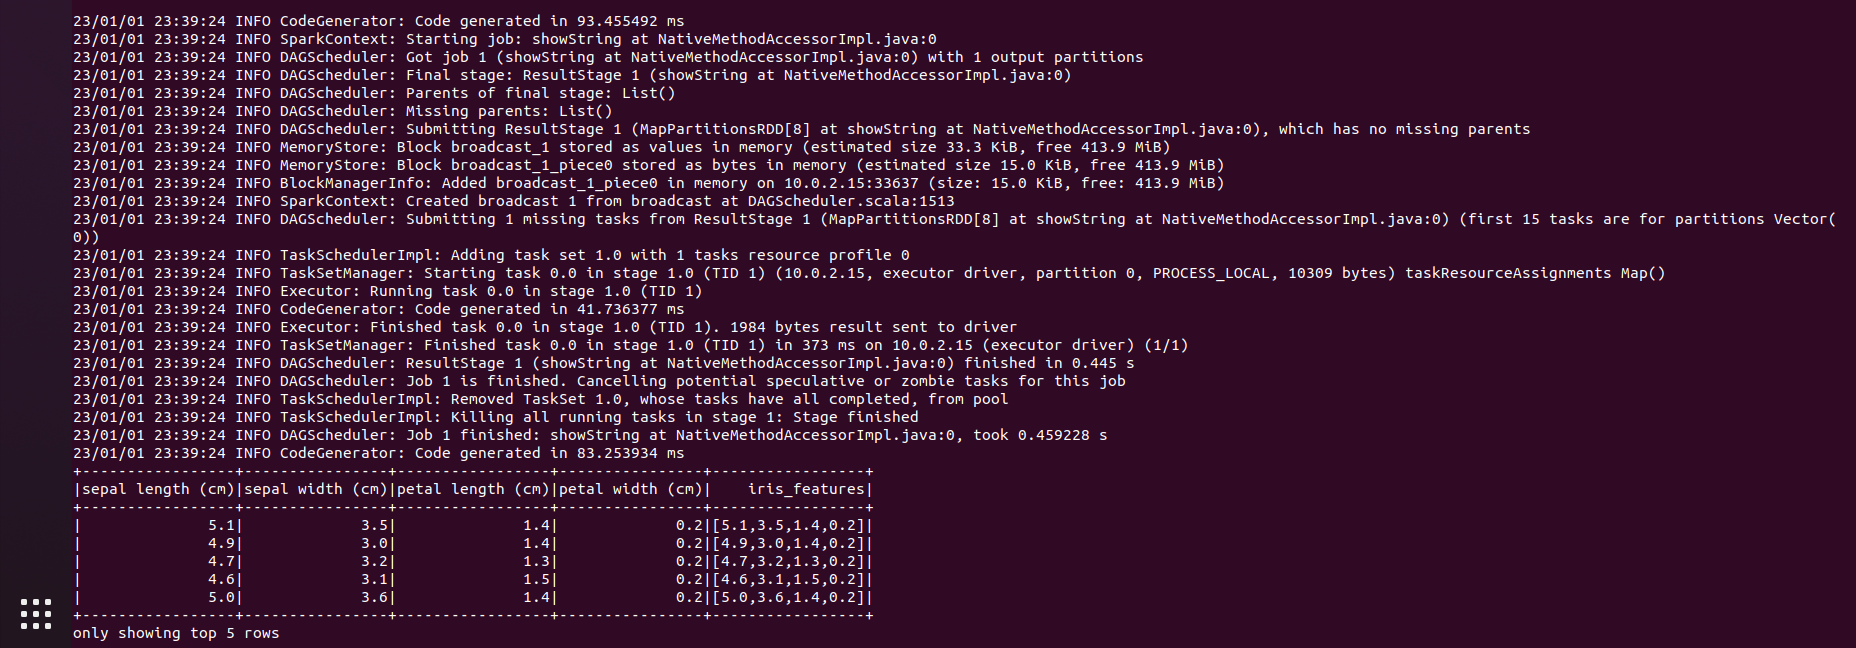
\includegraphics[width=.9\textwidth]{TugasKelompok/Kelompok4/tabelkedua}
\caption{vektor bunga iris yang dihasilkan dari ciri-ciri yang telah diinput}
\label{gam:perkuliahan-23-09}
\end{figure}
\newpage
\begin{figure}[!ht]
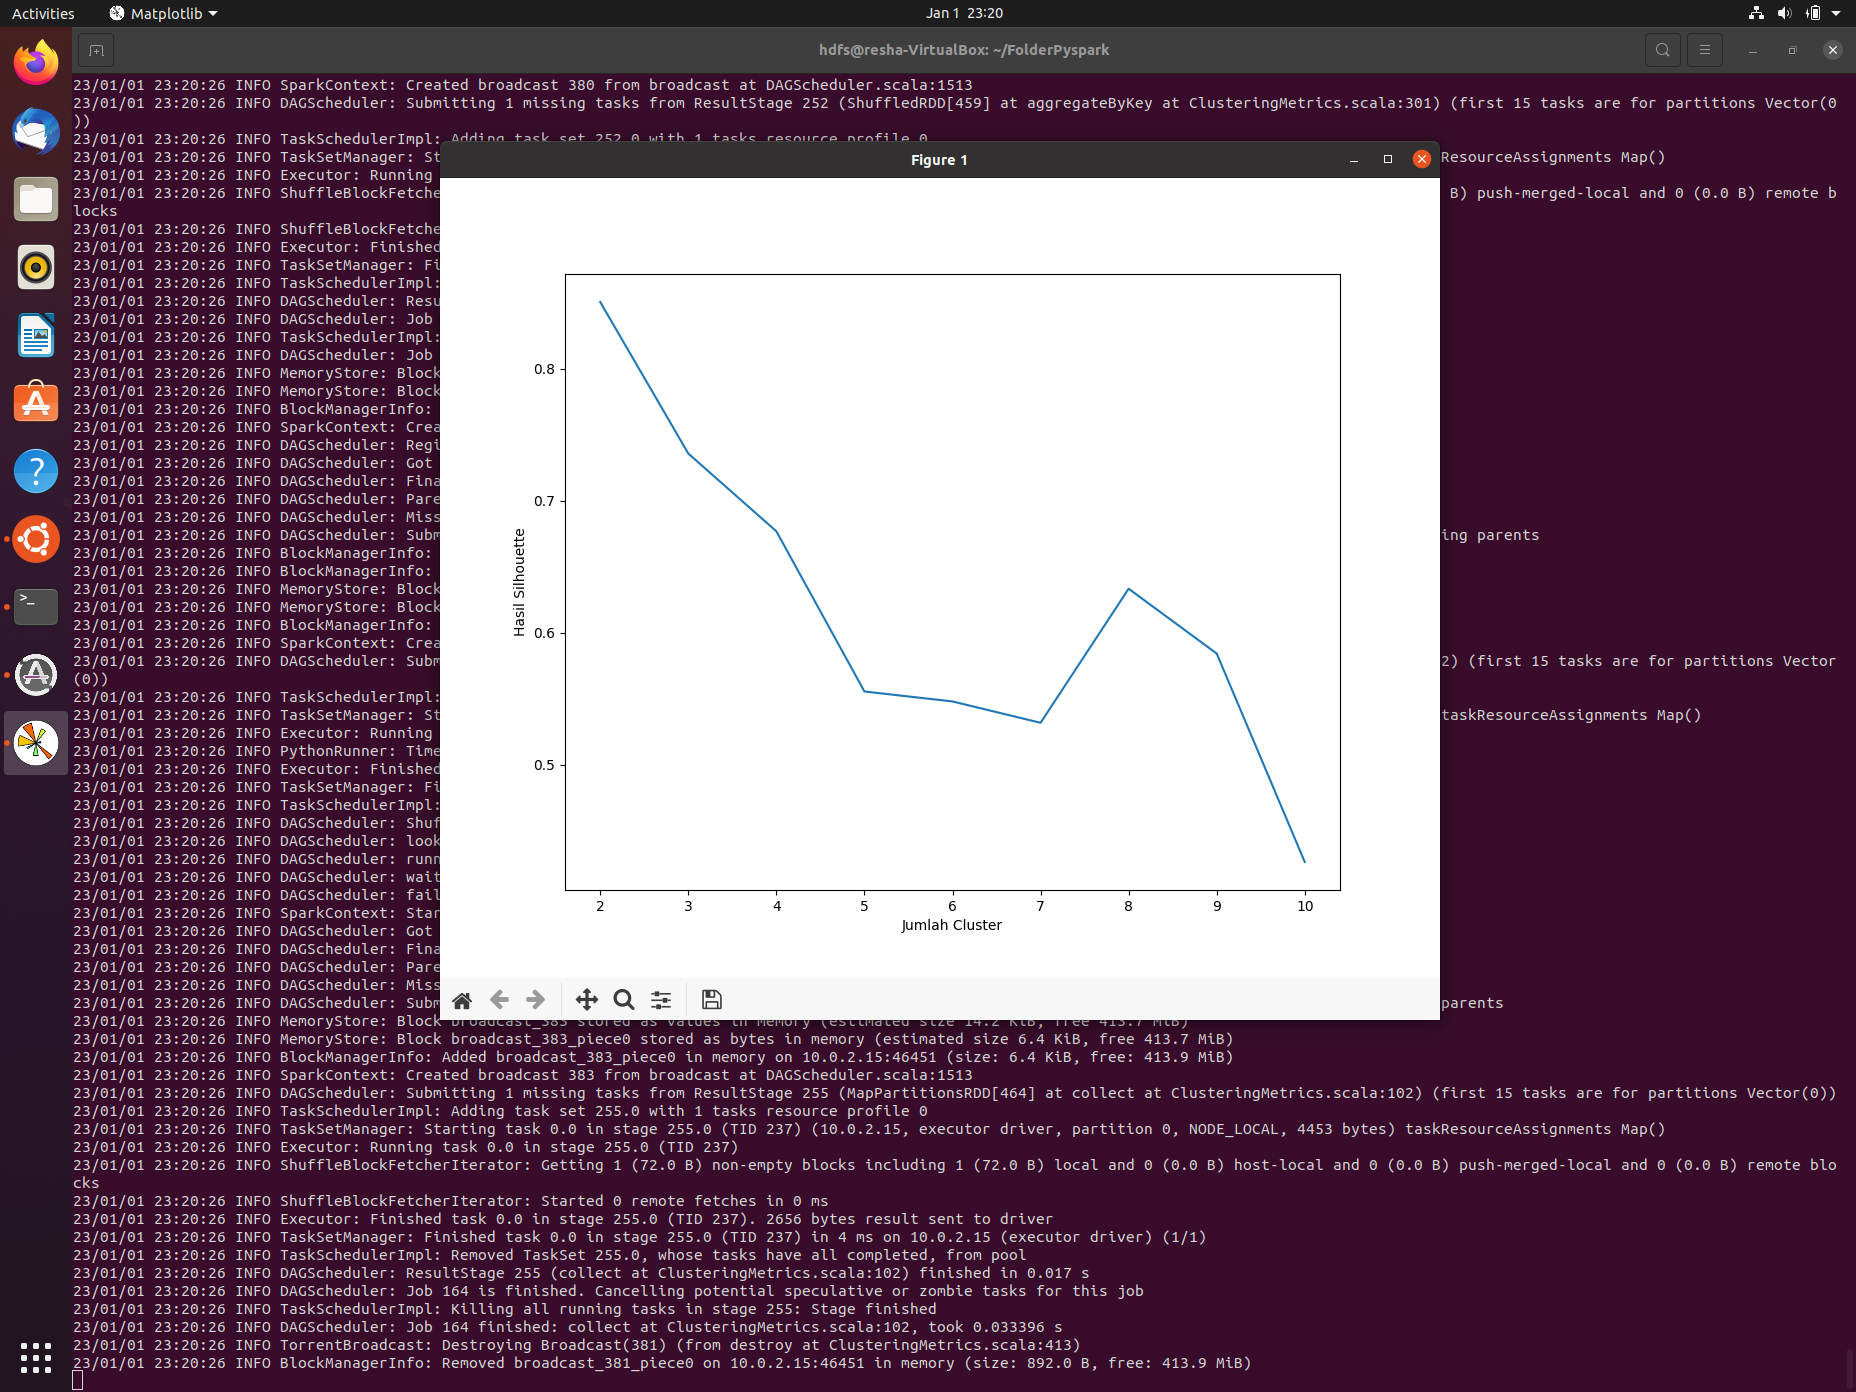
\includegraphics[width=.8\textwidth]{TugasKelompok/Kelompok4/grafikpertama}
\caption{grafik jumlah cluster dan hasil silhouette dari software metaploit}
\label{gam:perkuliahan-23-09}
\end{figure}
\begin{figure}[!ht]
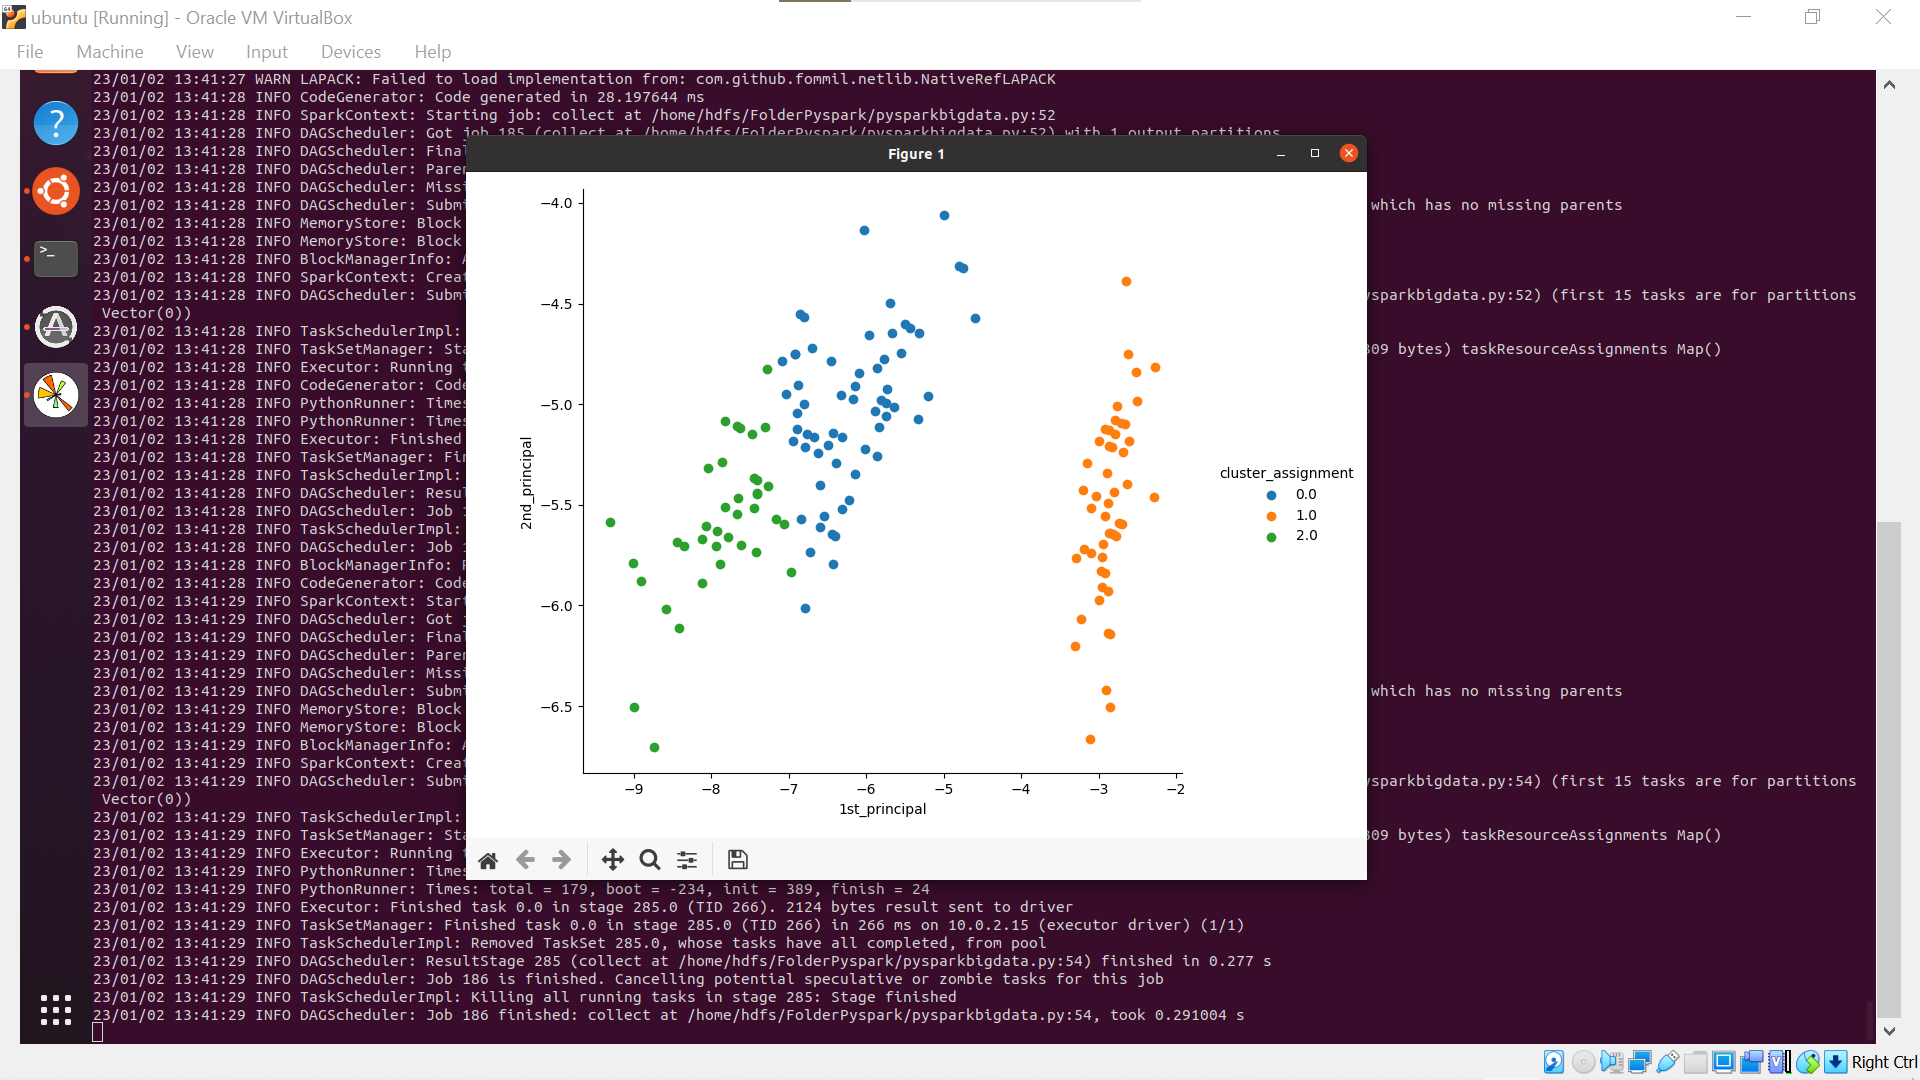
\includegraphics[width=.8\textwidth]{TugasKelompok/Kelompok4/grafikkedua}
\caption{grafik cluster assignment dari software metaploit}
\label{gam:perkuliahan-23-09}
\end{figure}

\end{enumerate}